\chapter{Generated Test Benchmarking}\label{chap:generated-benchmarking}
The evaluation of decision procedures for logical systems requires comprehensive and representative test suites to accurately assess their performance characteristics.
As shown in Chapter~\ref{chap:tptp-benchmarking}, our initial benchmarking using the TPTP library revealed a significant limitation: the scarcity of adequate test cases for fluted logic problems.
While TPTP serves as a valuable resource for many logical systems, the insufficient number of fluted logic examples prevented thorough performance evaluation of our implementation.

To address this limitation identified in the previous chapter, we developed an automated test case generation system specifically designed for fluted logic problems.
This approach allows us to create a large, diverse set of test instances with controllable parameters, enabling systematic evaluation of our decision procedure under various conditions and problem characteristics.

This chapter presents a comprehensive benchmarking study of our fluted logic decision procedure implementation.
We begin by describing the design and development of our automated test generator, explaining the rationale behind our chosen generation strategies and the parameters that control problem complexity and structure.
Subsequently, we detail our experimental methodology, including the selection of parameter ranges and the rationale for our benchmarking approach.
Finally, we present and analyse the performance results, examining how different problem characteristics affect the efficiency and scalability of our implementation.
The automated generation approach not only addresses the immediate need for adequate test cases identified in the last chapter but also provides a foundation for reproducible evaluation and future comparative studies in fluted logic decision procedures.
Through this systematic benchmarking, we aim to provide insights into the practical performance characteristics of our implementation in comparison to Vampire.
\section{Fluted Generator}\label{sec:fluted-generator}


\subsection{Design and Architecture}\label{subsec:design-and-implementation}
As for the \code{Classifier} class in Chapter~\ref{chap:tptp-benchmarking}, the \code{FlutedGenerator} class is implemented leveraging Vampire's existing infrastructure, both to facilitate the integration with the solver and to use its detailed first-order problem representation described in Section~\ref{sec:problems-representation}.
We also decided to narrow the generation only to FOF problems, this is to test the preprocessing to the maximum, which is not involved in the resolution of CNF problems, and to accelerate the implementation and proceed as soon as possible to testing.
The construction of fluted formulae is in fact quite straightforward, being that the only constraint to be respected is on the sequence of variables, unlike the fluted clauses that have multiple possible options, which can become quite complex to fairly randomly generate.

The idea is to build the formula recursively, descending its syntactic tree, and at each step randomly choosing which logical construct to use, until reaching the leaves of the tree, which correspond to the atomic formulae.
Given a fixed number of variables \(m\), which constitutes the set \(X_m\), to ensure that the generated formula is fluted, it suffices to build it following the top-down approach described in Section~\ref{sec:fluted-formulae}, where at each step, if a quantifier is chosen, a new variable is added to the sequence of available variables, until reaching the maximum \(m\).
To ensure that the generated formula is a sentence and with no 0-ary predicates, \(m\) has to be greater than 0 and equal to the maximum arity of the predicates used in the formula.
This \(m\) is therefore the first parameter of the generator, which we will refer to as \emph{maximal arity} or \code{_maxArity} in the code.

To simplify the implementation, we limited \(\land\) and \(\lor\) to their binary versions, being equivalent to the \(n\)-ary ones, but allowing to the structure of the formula to be a binary tree instead of a more general one, and to unify the treatment of all logical connectives.
Talking about logical connectives, we also decided to exclude \(\implies\) as it can be expressed using \(\lnot\) and \(\lor\), and their presence would not add any expressive power to the formulae.
Biconditionals, on the other hand, were included, since their clausification produces two clauses, and therefore their number of occurrences affects directly the preprocessing phase and the size of the set of clauses to be saturated.
Indeed, as mentioned in Section~\ref{sec:tptp-results-analysis}, one of the problem where Vampire outperformed our implementation with \emph{LRS} (SYN007+1) was due to the presence of many biconditionals in the original formula.
The probability of choosing each logical connective once a binary formula is to be generated are other parameters of the generator, which we will refer to as \emph{connectives' distribution} or \code{_andProb}, \code{orProb} and \code{iffProb} in the code.
These parameters are checked to form a probability distribution during initialization, and if some of them are not specified, they uniformly distribute the remaining probability mass.
Moreover, we limited negation to be applied inside atomic formulae only, allowing to take into account of those only when arriving at the leaves of the syntactic tree, where atomic formulae are generated.

To further control the complexity of the generated formula, we needed a bound on its size.
This is to avoid the occurrence of numerous consecutive logical connective extractions, leading to syntactic trees that would be uncontrollably diverse in size, ranging from trivially small atomic formulae to exponentially large nested structures that would render systematic testing infeasible.
For doing so, two approaches were possible: either limit the height of the syntactic tree (the depth of the formula) or the number of nodes in it (the length in symbols of the formula).
At first, we opted for the former, as it seemed more intuitive for a tree structure. After more refining though, we realized that the latter was more suited for our purposes, as it can more easily allow generating unbalanced trees, which are more likely to occur in real-world problems.
This parameter will be referred to as \emph{maximal length} or \code{_maxLen} in the code.

Another important aspect to consider is that resolution needs clauses containing unifiable literals to make progress. Therefore, predicates could not be generated every time a new atomic formula is created, but they had to be selected from a pool of previously generated predicates.
For doing this, we introduced a parameter that controls the number of distinct predicate names per arity, which we will refer to as \emph{predicates number} or \code{_predNum} in the code.

Furthermore, another parameter was need to control the number of units generated, which we will refer to as \emph{units number} or \code{_unitsNum} in the code.

Lastly, to allow reproducibility of the generated problems, a seed for the random number generator can be specified, which we will refer to as \emph{random seed} or \code{_seed} in the code.
If no seed is specified, standard C++ randomization techniques will be used.

All these parameters are given during the initialization of the generator and can be adjusted to control the characteristics of the generated problems.

\begin{figure}[H]
  \centering
  
\includegraphics[width=0.8\textwidth]{Placeholder.png}
  \caption{Class diagram of the \code{FlutedGenerator} Class.}\label{fig:fluted-generator-architecture}
\end{figure}

\subsection{Random choices distributions}\label{subsec:random-choices-distributions}

Choosing the right distributions for the random samplings is crucial to ensure that the generated problems are diverse and representative of real-world scenarios.
For doing this, we used C++'s \code{<random>} library, which provides a variety of random number generators and distributions.
To improve code quality and reusability, we encapsulated the random sampling functionalities in helpers methods within the \code{FlutedGenerator} class.

The first distribution used for sampling is the uniform distribution \(\mathcal{U}(A,B)\) on a discrete range.
\begin{figure}[H]
  \centering
  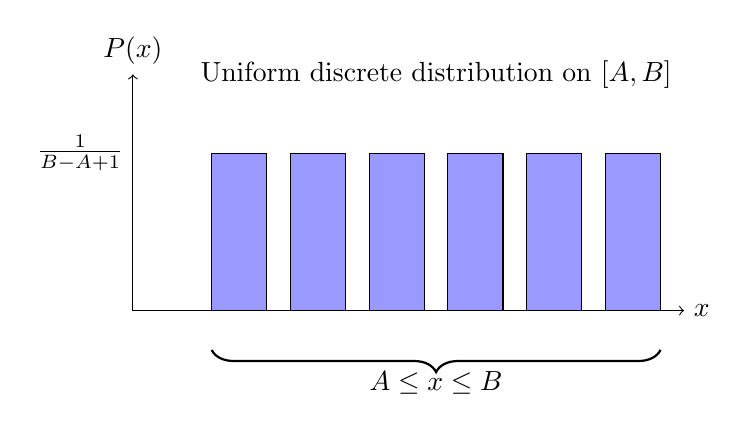
\begin{tikzpicture}
    % Parameters
    \def\a{2}
    \def\b{7}
    \def\n{\b-\a+1}
    \def\height{2}

    % Axes
    \draw[->] (\a-1,0) -- (\b+1,0) node[right] {\(x\)};
    \draw[->] (\a-1,0) -- (\a-1,3) node[above] {\(P(x)\)};

    % Bars for uniform discrete distribution from A to B
    \foreach \x in {\a,...,\b}
      \draw[fill=blue!40] (\x,0) rectangle (\x+0.7,\height);


    % Probability value
    \node[left] at (\a-1,\height) {\(\frac{1}{B-A+1}\)};

    % Title
    \node[above] at ({(\a+\b)/2+0.35},2.7) {Uniform discrete distribution on $[A,B]$};

    % Interval annotation
    \draw[decorate,decoration={brace,amplitude=8pt,mirror},thick] (\a, -0.5) -- (\b+0.7, -0.5) node[midway,below,yshift=-4pt] {\(A \leq x \leq B\)};
  \end{tikzpicture}
  \caption{Uniform discrete distribution over the integers from \(A\) to \(B\)}\label{fig:uniform-discrete-distribution-interval}
\end{figure}

This distribution is used in almost all the random samplings which require a choice from a discrete range of options, such as selecting a predicate from the pool of available ones.
The choice of which logical connective to use instead is made using the discrete distribution given by the \emph{connectives' distribution} parameters. If none of them is specified, the uniform distribution is used instead.

\begin{figure}[H]
  \centering
  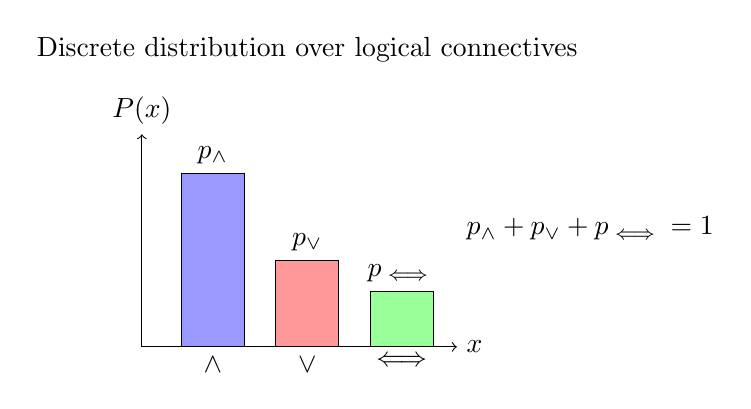
\begin{tikzpicture}
    % Parameters
    \def\heightAnd{2.2}
    \def\heightOr{1.1}
    \def\heightIff{0.7}
    \def\width{0.8}

    % Axes
    \draw[->] (-0.5,0) -- (3.5,0) node[right] {\(x\)};
    \draw[->] (-0.5,0) -- (-0.5,2.7) node[above] {\(P(x)\)};

    % Bars
    \draw[fill=blue!40] (0,0) rectangle (\width,\heightAnd);
    \draw[fill=red!40] (1.2,0) rectangle (1.2+\width,\heightOr);
    \draw[fill=green!40] (2.4,0) rectangle (2.4+\width,\heightIff);

    % Labels below bars
    \node[below] at (0+\width/2,0) {\(\land\)};
    \node[below] at (1.2+\width/2,0) {\(\lor\)};
    \node[below] at (2.4+\width/2,0) {\(\iff\)};

    % Probability values above bars
    \node[above] at (0+\width/2,\heightAnd) {\(p_{\land}\)};
    \node[above] at (1.2+\width/2,\heightOr) {\(p_{\lor}\)};
    \node[above] at (2.4+\width/2,\heightIff) {\(p_{\iff}\)};

    % Title
    \node[above] at (1.2+\width/2,3.5) {Discrete distribution over logical connectives};

    % Sum annotation
    \node[right] at (3.5,1.5) {\(p_{\land} + p_{\lor} + p_{\iff} = 1\)};
  \end{tikzpicture}
  \caption{Example of a discrete probability distribution over logical connectives}\label{fig:connectives-discrete-distribution}
\end{figure}

For binary samplings, such as deciding whether to negate an atomic formula or which quantifier to use, we used the Bernoulli distribution \(\mathcal{B}(p)\), where \(p\) has been fine-tuned for each specific case.

\begin{figure}[H]
  \centering
  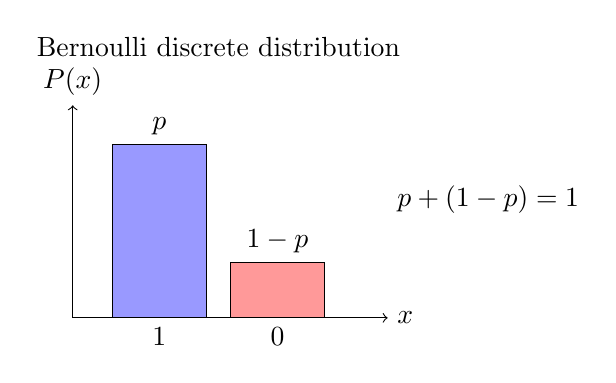
\begin{tikzpicture}
    % Parameters
    \def\width{1.2}
    \def\heightOne{2.2}
    \def\heightZero{0.7}

    % Axes
    \draw[->] (-0.5,0) -- (3.5,0) node[right] {\(x\)};
    \draw[->] (-0.5,0) -- (-0.5,2.7) node[above] {\(P(x)\)};

    % Bars
    \draw[fill=blue!40] (0,0) rectangle (\width,\heightOne);
    \draw[fill=red!40] (1.5,0) rectangle (1.5+\width,\heightZero);

    % Labels below bars
    \node[below] at (0+\width/2,0) {\(1\)};
    \node[below] at (1.5+\width/2,0) {\(0\)};

    % Probability values above bars
    \node[above] at (0+\width/2,\heightOne) {\(p\)};
    \node[above] at (1.5+\width/2,\heightZero) {\(1-p\)};

    % Title
    \node[above] at (0.75+\width/2,3.2) {Bernoulli discrete distribution};

    % Sum annotation
    \node[right] at (3.5,1.5) {\(p + (1-p) = 1\)};
  \end{tikzpicture}
  \caption{Bernoulli discrete distribution with parameter \(p\).}\label{fig:bernoulli-discrete-distribution}
\end{figure}

Lastly, there was another occasion of random sampling not yet covered.
After choosing to generate a binary formula, to increase the variability of the structures of the generated trees, we decided to randomly choose how many symbols to allocate to the left and right subformulae.
This is done by sampling a real coefficient \(c\) from a normal distribution \(\mathcal{N}(\mu, \sigma^2)\) with mean \(\mu = 0.5\) and standard deviation \(\sigma = \frac{1}{18}\), which is then used to proportionally split the available symbols between the two subformulae.
This value of \(\sigma\) was chosen to ensure that the vast majority of the sampled values fall within the range \([\frac{1}{3}, \frac{2}{3}]\), thus avoiding excessively unbalanced splits.
Furthermore, avoiding sampling outside a specified range is mandatory, due to the discrete nature of the length parameter, which would not allow allocating at least one symbol to each subformula.
The natural base case of the recursion, which occurs when the length is \(3\), where the only possible split is 1 symbol for one subformula and 1 for the other, with the remaining symbol being used for the connective.
Being the number of symbols always greater than \(3\) when sampling this coefficient, we can safely use the range \([\frac{1}{3}, \frac{2}{3}]\) for sampling, as it guarantees that both subformulae will always receive at least one symbol.
To achieve this, we implemented a rejection sampling approach, where values outside the specified range are discarded and resampled until a valid value is obtained.
The values of \(\mu\) and \(\sigma\) were chosen to ensure that the vast majority of the sampled values fall within the desired range, thus minimizing the number of rejections and ensuring efficient sampling.

\begin{figure}[H]
  \centering
  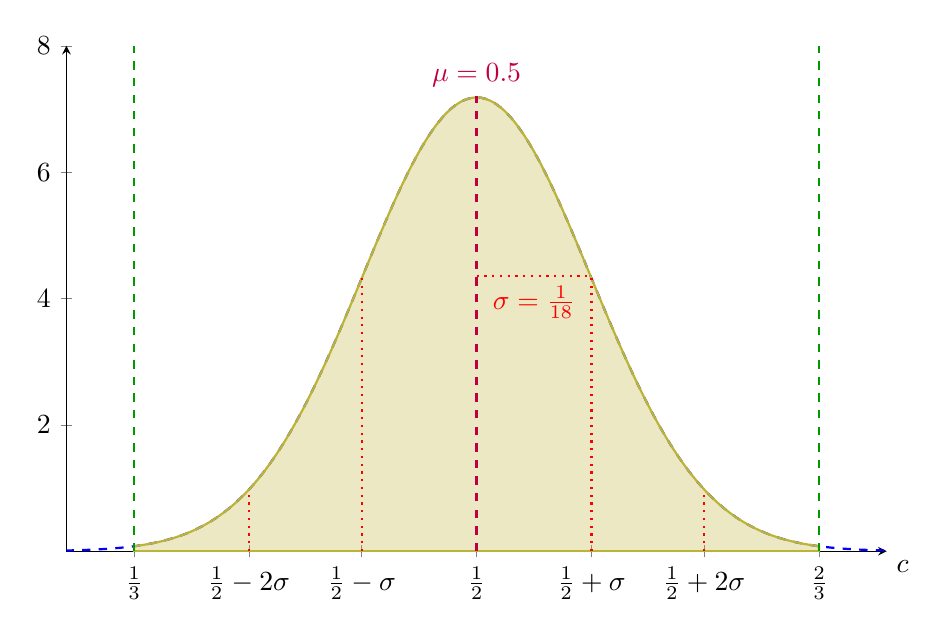
\begin{tikzpicture}
\begin{axis}[
    width=12cm,
    height=8cm,
    axis lines=middle,
    xlabel={$c$},
    xlabel style={at={(axis description cs:1,0)}, anchor=north west},
    ylabel style={at={(axis description cs:0,1)}, anchor=south east, rotate=90},
    xmin=0.3, xmax=0.7,
    ymin=0, ymax=8,
    xtick={0, 0.333,0.389,0.444, 0.5, 0.556, 0.611, 0.667, 1},
    xticklabels={0, $\frac{1}{3}$,$\frac{1}{2}-2\sigma$,$\frac{1}{2}-\sigma$, $\frac{1}{2}$,$\frac{1}{2}+\sigma$,$\frac{1}{2}+2\sigma$, $\frac{2}{3}$, 1},
    ytick={0, 2, 4, 6, 8},
    legend pos=north east,
    title style={font=\large\bfseries}
]

% Distribuzione normale originale (non troncata)
\addplot[
    domain=0:1,
    samples=200,
    smooth,
    thick,
    blue,
    dashed
] {1/sqrt(2*pi*(1/18)^2) * exp(-0.5*((x-0.5)/(1/18))^2)};

% Area troncata (parte accettata)
\addplot[
    domain=0.333:0.667,
    samples=100,
    smooth,
    thick,
    yellow!70!black,
    fill=yellow!70!black,
    fill opacity=0.3
] {1/sqrt(2*pi*(1/18)^2) * exp(-0.5*((x-0.5)/(1/18))^2)} \closedcycle;

% Linee verticali per i limiti di troncamento
\draw[thick, green!60!black,dashed] (axis cs:0.333,0) -- (axis cs:0.333,8);
\draw[thick, green!60!black,dashed] (axis cs:0.667,0) -- (axis cs:0.667,8);

% Linea verticale per la media
\draw[thick, purple, dashed] (axis cs:0.5,0) -- (axis cs:0.5,7.2);

\draw[thick, red, dotted] (axis cs:0.556,0) -- (axis cs:0.556,4.355);
\draw[thick, red, dotted] (axis cs:0.5,4.355) -- (axis cs:0.556,4.355);
\node[anchor=north, red] at (axis cs:0.528, 4.355) {$\sigma = \frac{1}{18}$};
% μ - σ = 0.5 - 1/18 ≈ 0.444  
\draw[thick, red, dotted] (axis cs:0.444,0) -- (axis cs:0.444,4.355);

% μ + 2σ = 0.5 + 2/18 ≈ 0.611
\draw[thick, red, dotted] (axis cs:0.611,0) -- (axis cs:0.611,0.975);
% μ - 2σ = 0.5 - 2/18 ≈ 0.389
\draw[thick, red, dotted] (axis cs:0.389,0) -- (axis cs:0.389,0.975);

% Annotazioni
\node[anchor=south, purple] at (axis cs:0.5, 7.2) {$\mu = 0.5$};


% Legenda

\end{axis}

\end{tikzpicture}
  \caption{Normal distribution \(\mathcal{N}(0.5,\,{(\frac{1}{18})}^2)\) truncated to the interval \([\frac{1}{3}, \frac{2}{3}]\).}\label{fig:truncated-normal-distribution}
\end{figure}


\subsection{Generator Algorithms}\label{subsec:generator-algorithms}

The entry point method of the \code{FlutedGenerator} class is \code{generateProblem}, which generates a fluted problem according to the specified parameters.

\begin{algorithm}[H]
  \caption{Generate fluted problem}\label{alg:generate-fluted-problem}
  \begin{algorithmic}[1]
      \Statex{} \bold{signature} \(\textsc{generateProblem:} \quad Void \to Boolean\)
      \Function{\(\textsc{generateProblem}\)}{$ $} % chktex 46
        \State{} \(unitList \gets \emptyset\)
        \For{\(i \in \{1, \ldots, \_unitsNum\}\)}
          \State{} \(unit \gets generateUnit()\)
          \State{} \(unitList \gets unitList \cup \{unit\}\)
        \EndFor{}
        \State{} \Return{} \(Problem(unitList)\)
      \EndFunction{}
  \end{algorithmic}
\end{algorithm}


Its sole purpose is to call the \code{generateUnit} method the specified number of times, collecting the generated units in a list, and finally returning a \code{Problem} object containing them.
The \code{generateUnit} method is responsible for generating a single fluted \code{FormulaUnit}.
To try to generete more diverse and realistic problems, in this method a random number of usable variables, ranging from 1 to half of the maximum arity specified, is chosen to be quantified in advance.
This is to simulate the common situation in real-world problems where some variables are quantified at the beginning of the formula, as well as allowing proper formula generation to freely even literals from the start, having already some variables available.

\begin{algorithm}[H]
  \caption{Generate fluted unit}\label{alg:generate-fluted-unit}
  \begin{algorithmic}[1]
      \Statex{} \bold{signature} \(\textsc{generateUnit:} \quad Void \to Unit*\)
      \Function{\(\textsc{generateUnit}\)}{$ $} % chktex 46
        \State{} \(varNum \gets uniformRandom(1, \frac{\_maxArity}{2})\)
        \State{} \(usedVars \gets \{0,\ldots,varNum-1\}\)
        \State{} \(formula \gets generateFormula(\_maxLen-varNum, usedVars)\)
        \State{} \(usedVars \gets reverse(usedVars)\)
        \For{\(v \in usedVars\)}
          \State{} \(formula \gets randomlyQuantify(formula, v)\)
        \EndFor{}
        \State{} \Return{} \(FormulaUnit(formula)\)
      \EndFunction{}
  \end{algorithmic}
\end{algorithm}

To handle the generation of a specific type of subformula, being it atomic, binary, or quantified, some helper methods were implemented as follows:

\begin{algorithm}[H]
  \caption{Generate quantified formula}\label{alg:generate-quantified-formula}
  \begin{algorithmic}[1]
      \Statex{} \bold{signature} \(\textsc{randomlyQuantify:} \quad Formula* \times Var \to QuantifiedFormula*\)
      \Function{\(\textsc{randomlyQuantify}\)}{$f, v$} % chktex 46
        \State{} \(varList \gets \{v\}\)
        \If{\(bernoulliTrial(0.5)\)}
          \State{} \(quantifier \gets \exists\)
        \Else{}
          \State{} \(quantifier \gets \forall\)
        \EndIf{}
        \State{} \Return{} \(QuantifiedFormula(quantifier,varList, formula)\)
      \EndFunction{}
  \end{algorithmic}

\end{algorithm}
\begin{algorithm}[H]
  \caption{Generate atomic formula}\label{alg:generate-atomic-formula}
  \begin{algorithmic}[1]
      \Statex{} \bold{signature} \(\textsc{generateAtomicFormula:} \quad VList* \to AtomicFormula*\)
      \Function{\(\textsc{generateAtomicFormula}\)}{$usedVars$} % chktex 46
        \State{} \(arity \gets uniformRandom(1,usedVars)\)
        \State{} \(predIndex \gets uniformRandom(0, \_predNum - 1)\)
        \State{} \(predicate \gets \_predicates[arity-1] [predIndex]\)
        \State{} \(litVars \gets selectLastN(usedVars, arity)\)
        \State{} \(isNegated \gets bernoulliTrial(0.5)\)
        \State{} \(l \gets Literal(predicate, arity, isNegated,litVars)\)
        \State{} \Return{} \(AtomicFormula(l)\)
      \EndFunction{}
  \end{algorithmic}
\end{algorithm}
\begin{algorithm}[H]
  \caption{Generate binary formula}\label{alg:generate-binary-formula}
  \begin{algorithmic}[1]
      \Statex{} \bold{signature} \(\textsc{generateBinaryFormula:} \quad Unsigned \times VList* \to Formula*\)
      \Statex{} \textbf{require} \(len > 3\)
      \Function{\(\textsc{generateBinaryFormula}\)}{$len, usedVars$} % chktex 46
        \State{} \(connective \gets generateConnective()\)
        \Comment{Sampled from \emph{connectives' distribution}}
        \State{} \(remLen \gets len - 1\)
        \State{} \(c \gets truncatedNormalRandom(0.5, \frac{1}{18}, \frac{1}{3}, \frac{2}{3})\)
        \State{} \(leftLen \gets round(c \cdot remLen)\)
        \State{} \(rightLen \gets remLen - leftLen\)
        \State{} \(leftFormula \gets generateFormula(leftLen, usedVars)\)
        \State{} \(rightFormula \gets generateFormula(rightLen, usedVars)\)
        \If{\(connective = \iff\)}
          \State{} \Return{} \(BinaryFormula(\iff,leftFormula, rightFormula)\)
        \Else{}
          \State{} \Return{} \(JunctionFormula(connective,\{leftFormula, rightFormula\})\)
        \EndIf{}
      \EndFunction{}
  \end{algorithmic}
\end{algorithm}

Finally, the \code{generateFormula} method orchestrates the recursive generation of the formula, deciding at each step which type of subformula to generate based on the remaining length and the available variables.
To chose if generating a quantified formula or not, we used a Bernoulli distribution with \(p\) dynamically adjusted with the function
\[
p_{quantify} = \min\left(\frac{\_maxArity - |usedVars|}{remainingLength - 1}, 1\right)
\]
\begin{figure}[H]
\centering
\begin{minipage}{0.48\textwidth}
\centering
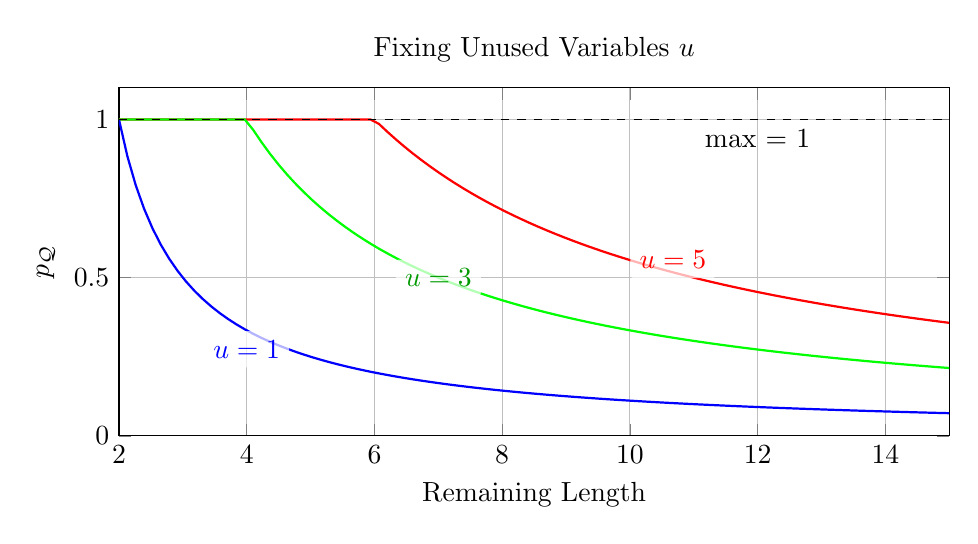
\begin{tikzpicture}
\begin{axis}[
    xlabel={Remaining Length},
    ylabel={$p_{\mathcal{Q}}$},
    xmin=2, xmax=15,
    ymin=0, ymax=1.1,
    grid=major,
    width=\textwidth,
    height=6cm,
    samples=100,
    title={Fixing Unused Variables \(u\)}
]

\addplot[red, thick, domain=2:15] {min(5/(x-1), 1)};
\addplot[green, thick, domain=2:15] {min(3/(x-1), 1)};
\addplot[blue, thick, domain=2:15] {min(1/(x-1), 1)};
\addplot[black, dashed, domain=2:15] {1};

\node[blue, anchor=north, fill=white, fill opacity=0.7, text opacity=1, rounded corners=1pt] at (axis cs:4, 0.333) {\(u = 1\)};
\node[green!60!black, fill=white, fill opacity=0.7, text opacity=1, rounded corners=1pt] at (axis cs:7, 0.5) {\(u = 3\)};
\node[red, anchor=west, fill=white, fill opacity=0.7, text opacity=1, rounded corners=1pt] at (axis cs:10, 0.556) {\(u = 5\)};
\node[black, anchor=north] at (axis cs:12, 1) {max = 1};

\end{axis}
\end{tikzpicture}

\end{minipage}
\hfill
\begin{minipage}{0.48\textwidth}
\centering
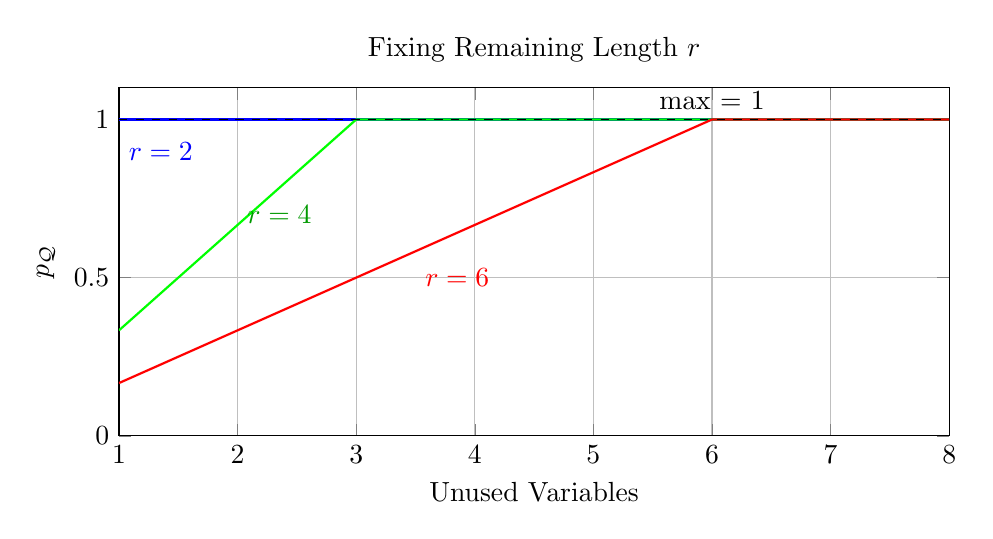
\begin{tikzpicture}
\begin{axis}[
    xlabel={Unused Variables},
    ylabel={$p_{\mathcal{Q}}$},
    xmin=1, xmax=8,
    ymin=0, ymax=1.1,
    grid=major,
    width=\textwidth,
    height=6cm,
    samples=100,
    title={Fixing Remaining Length \(r\)}
]

\addplot[blue, thick, domain=1:10] {min(x/1, 1)};
\node[blue, anchor=west] at (axis cs:1, 0.9) {\(r = 2\)};

\addplot[green, thick, domain=1:10] {min(x/3, 1)};
\node[green!60!black, anchor=west] at (axis cs:2, 0.7) {\(r = 4\)};


\addplot[red, thick, domain=1:10] {min(x/6, 1)};
\node[red, anchor=west] at (axis cs:3.5, 0.5) {\(r = 6\)};

\addplot[black, dashed, domain=1:10] {1};
\node[black, anchor=south] at (axis cs:6, 1) {max = 1};

\end{axis}
\end{tikzpicture}

\end{minipage}
\caption{Behaviour of \(p_{\mathcal{Q}}\) with fixed unused variables (left) and fixed remaining length (right).}\label{fig:pquantify}
\end{figure}

This function ensures that the probability of quantifying a new variable increases as the density of quantification in the formula decreases, thus promoting a balanced distribution of quantifiers throughout the formula.

Finally, the \code{generateFormula} method is as follows:
\begin{algorithm}[H]
  \caption{Generate fluted formula}\label{alg:generate-fluted-formula}
  \begin{algorithmic}[1]
      \Statex{} \bold{signature} \(\textsc{generateFormula:} \quad Unsigned \times VList* \to Formula*\)
      \Statex{} \textbf{require} \(len \geq 3\)
      \Function{\(\textsc{generateFormula}\)}{$len, usedVars$} % chktex 46
        \If{\(len = 1\)}
          \State{} \Return{} \(generateAtomicFormula(usedVars)\)
        \EndIf{}
        \State{} \(varNum \gets |usedVars|\)
        \If{\(varNum \geq \_maxArity\)}
        \Comment{No quantification possible}
          \If{\(len = 2\)}
            \Comment{Cannot generate binary formula}
            \State{} \Return{} \(generateAtomicFormula(usedVars)\)
          \EndIf{}
        \Else{}
          \State{} \(p_{\mathcal{Q}} \gets \min\left(\frac{\_maxArity - varNum}{len - 1}, 1\right)\)
          \If{\(bernoulliTrial(p_{\mathcal{Q}})\)}
            \Comment{Generate quantified formula}
            \State{} \(usedVars \gets usedVars \cup \{varNum\}\)
            \State{} \(subFormula \gets generateFormula(len - 1, usedVars)\)
            \State{} \Return{} \(randomlyQuantify(subFormula, varNum)\)
          \EndIf{}
        \EndIf{}
        \If{\(bernoulliTrial(0.1)\)}
          \Comment{Rare premature atomic formula generation}
          \State{} \Return{} \(generateAtomicFormula(usedVars)\)
        \Else{}
          \Comment{Generate binary formula}
          \State{} \Return{} \(generateBinaryFormula(len, usedVars)\)
        \EndIf{}
      \EndFunction{}
  \end{algorithmic}
\end{algorithm}

Due to time constraints, we decided to limit the generation to unsatisfiable problems only, to have easier and more reliable means of verifying the correctness of the implementation, allowing for more controlled testing conditions.
To achieve this, we implemented a simple strategy: for each generated problem, a random unit is selected, and its negation is added to the problem as an additional unit.

To have more variety and to try to decrease the instant resolutions, we considered the possibility of altering the unit to be negated before adding it to the list, substituting a section of the initial sequence of quantifiers with existential quantifiers.
However, this idea was not implemented in the current work, and we leave it as a direction for future improvements and experiments.
\section{Generation Parameters}\label{sec:generation-parameters}

To conduct a systematic benchmarking study, we had to decide which generation parameters could significantly impact the performance of the decision procedures and therefore should be varied during the experiments.
Other than this, we also had to choose appropriate ranges for these parameters, balancing the need for diversity in the generated problems with the practical constraints of computational resources and time.
After careful consideration, we identified the following key parameters to vary:
\begin{itemize}
\item \textbf{Maximal arity} (\code{_maxArity}):  This parameter is fundamental, as it directly controls the maximum number of variables \(m\) that can appear in a generated formula.
                                                  Since the satisfiability problem for the fluted fragment is known to have \emph{non-elementary complexity} in \(m\)~\cite{pratt2019fluted}, with the fluted formula over \(m\) variables being
                                                   \(\lfloor \frac{m}{2} \rfloor-\textsc{NExpTime}\)-hard and requiring models of \((\frac{m}{2})\)-tuply exponential size, \code{_maxArity} is expected to have a significant impact on performance.
                                                  We chose to vary this parameter from \(2\) to \(15\), to cover a wide range of complexities while keeping the generated problems manageable for testing.
\item \textbf{Maximal length} (\code{_maxLen}): This parameter controls the size of the generated formulae, which can affect both the preprocessing time and the saturation time.
                                                Moreover, longer formulae can lead to a larger number of clauses after clausification, potentially increasing the search space for the resolution procedure.
                                                On the other hand, increasing the number of clauses produced can also provide more opportunities for contradictions to be generated, which could potentially aid in finding a refutation.
                                                We decided to vary this parameter from \(10\) to \(30\) with increments of \(5\).
\item \textbf{Predicates number} (\code{_predNum}): This parameter influences the diversity of predicates in the generated formulae.
                                                  A higher number of distinct predicates can lead to fewer opportunities for unification during resolution, potentially increasing the difficulty of the problem.
                                                  We chose to vary this parameter from \(1\) to \(10\) to observe its effect on performance.
\item \textbf{Units number} (\code{_unitsNum}): This parameter determines the number of units in the generated problem.
                                                Similarly to the maximal length, increasing the number of units can lead to a larger search space, but also more opportunities for contradictions.
                                                We decided to vary this parameter from \(1\) to \(10\) with gaps of \(3\).
\item \textbf{Connectives' distribution} (\code{_iffProb}): As shown in Section~\ref{sec:tptp-results-analysis}, the presence of biconditionals can significantly affect the performance of the fluted preprocessing and resolution.
                                                            To study this effect, we decided to vary the probability of generating biconditionals (and consequently the probabilities of generating conjunctions and disjunctions) in the generated formulae.
                                                            We chose to have three different options for this parameter: \(\frac{1}{3}\), \(\frac{2}{5}\), and \(\frac{1}{2}\), with the remaining probability mass distributed uniformly between conjunctions and disjunctions.

\end{itemize}
\subsection{Gradual difficulty escalation}\label{subsec:gradual-difficulty-escalation}

Combining all the variations of the selected parameters would lead to a total of \(14 \times 5 \times 10 \times 4 \times 3 = 8400\) different configurations.
To add more robustness to the experiments, we decided to generate \(25\) instances for each configuration, leading to a total of \(210000\) generated problems.

With so many problems to test, it was crucial to have a systematic approach to manage how parameters were varied to avoid growing the complexity of the problems too quickly on one axis while neglecting others.
Iterating through all the combinations in a naive way could lead to situations where some parameters were increased too rapidly, resulting in problems that were too difficult to solve within the time limits, while others remained too easy.
To address this, we implemented a gradual difficulty escalation strategy, where parameters were increased in a controlled manner.

First, we identified the parameters that we expected to have the least impact on the complexity of the problems: \code{_predNum}, \code{_maxLen}, and \code{_unitsNum}.
Those three parameters were grouped together, and their combinations were iterated through in a nested manner.
In particular, these three parameters were encoded in three dimensions using a lexicographic ordering, with \code{_predNum} as the most significant dimension, \code{_maxLen} as the middle dimension, and \code{_unitsNum} as the least significant (i.e., the one that changes most rapidly).
In other words, the larger the domain of a parameter, the more slowly it was made to change, ensuring that variations in \code{_predNum} and \code{_maxLen} occur more gradually.
This strategy was chosen to provide immediate diversity in the generated instances, so that changes in the faster-varying parameter (\code{_unitsNum}) do not wait for a complete cycle of \code{_predNum} values (which has 10 possible values).

As mentioned above, variations in maximum arity were expected to have the most significant impact on problem complexity, so we opted to vary this parameter at the same rate as the combination of the previous 3.
For doing so, we encoded the values of the previous 3 parameters into a single index \(i\) ranging from \(0\) to \(199\) (the total number of combinations of the three parameters) using the formula
\[i = \text{\code{_predNum}} + \text{\code{_maxLen}} \times 4 + \text{\code{_unitsNum}} \times 20\]
Then, being \code{_maxArity} ranging from \(2\) to \(15\), we grouped the values of \(i\) into \(14\) groups, \(13\) of them containing \(15\) values and the last one containing \(5\) values.
Having now two equipotent sets of values, we could easily use Cantor's pairing function to combine them into a single index.
\[\pi(i, j) = \frac{(i + j)(i + j + 1)}{2} + j\]
This encoding ensures that as we iterate through the natural number, these can be decoded back into a pair of values \((i, j)\) that change in a balanced manner, thus achieving the desired gradual escalation of difficulty across all parameters.

\begin{figure}[H]
  \centering
  \begin{tikzpicture}[scale=0.7, transform shape]
    \begin{axis}[
      width=8cm,
      height=8cm,
      axis lines=middle,
      xlabel={$i$},
      ylabel={$j$},
      xlabel style={at={(axis description cs:0,1.05)}, anchor=west}, % etichetta x in alto
      ylabel style={at={(axis description cs:1.05,0)}, anchor=south},  % etichetta y a destra
      xmin=0, xmax=4,
      ymin=0, ymax=4,
      xtick={0,1,2,3,4},
      ytick={0,1,2,3,4},
      grid=both,
      minor tick num=0,
      tick label style={font=\small},
      title={Cantor Pairing Traversal}
    ]
      % Traversal arrows
      \addplot[thick, blue, -{Latex[length=2mm]}, mark=none] coordinates {
        (0,0) (0,1) (1,0) (0,2) (1,1) (2,0) (0,3) (1,2) (2,1) (3,0) (0,4) (1,3) (2,2) (3,1) (4,0)
      };

    \foreach \s in {0,...,4} {
      \foreach \k in {0,...,4} {
        \pgfmathsetmacro{\i}{\k}
        \pgfmathsetmacro{\j}{\s-\k}
        \pgfmathsetmacro{\cantor}{(\i+\j)*(\i+\j+1)/2+\j}
        \addplot[ only marks] coordinates {(\i,\j)};
      }
    }
    \end{axis}
    % Cantor pairing traversal (diagonals) con etichette

  \end{tikzpicture}
  \caption{Traversal order of the Cantor pairing function: diagonal progression \((0,0)\to(0,1)\to(1,0)\to(0,2)\to(1,1)\to(2,0)\to\cdots\) on the \(i,j\) plane.}\label{fig:cantor-pairing-diagonal}
\end{figure}

Finally, the probability of generating biconditionals was varied at the slowest rate, changing only after a complete cycle of the previous 4 parameters.

\section{Experimental Setup, Results and Analysis}\label{sec:results-analysis}

For the generated problems testing, we used a similar experimental setup to the one used for the TPTP problems, with some differences.
The hardware used for the tests was the same as described in Section~\ref{sec:tptp-experimental-setup}, as well as time limit of \(300\) seconds per problem and the symbolic value of \(330\) for problems which led to an error.

For measuring the impact of the preprocessing step, we decided to include a new hybrid execution mode, where the fluted preprocessing is applied, but the resulting clauses are then passed to the standard non-fluted resolution procedure.
This hybrid mode allows us to isolate the effect of the preprocessing step from the fluted-specific optimizations in the resolution procedure, providing a clearer picture of where the performance gains are coming from.

As for the resolution strategy, in this case we limited ourselves to the \emph{LRS} strategy, since its performance are typically better. Its incompleteness is not a concern here, as we are only dealing with unsatisfiable problems.
In any case, all the problems that resulted satisfiable by the LRS strategy were flagged as errors, and accumulated in a log for future further analysis.

Testing all the huge number of generated problems we aimed to test (\(210000 \times 3\) modes = \(630000 \times 5\) runs = \(3150000 \times 5\) potential minutes = \(15750000\) minutes), was simply not feasible as it would have required potentially nearly 30 years of continuous computation.
To make the experiments manageable, we decided to do multiple runs only to problems that took less than \(30\) seconds in the first run, where possible hardware or software fluctuations could have a more significant impact on the measured time.
Moreover, after some initial experimentation that highlighted the fact that the timeout of hybrid mode and Vampire mode were very similar, we decided to skip Vampire mode for problems that reached the timeout in hybrid mode, as they were very likely to also timeout in Vampire mode.
For those problems, a symbolic value of \(400\) seconds was assigned to Vampire mode for charts, while a value of \(300\) seconds was assigned when calculating aggregated results.

Although the tests have performed at any time possible for over two months, we managed to complete only the first \(75/200\) numbers of lexicographic encoding for the first \(8/14\) variables, never changing the value of \code{_iffProb} from \(\frac{1}{3}\).
This resulted in a total of \(15000\) generated problems, which were tested in all three modes, leading to a total of \(45000\) tests, potentially with \(5\) runs each.
The full set of results was too large to be included in this document, so we uploaded it to a public repository\footnote{\url{https://github.com/RiccardoElena/thesis_benchmarks}}.
Even reporting charts similar to those in Section~\ref{sec:tptp-results-analysis} with all problems on the x-axis would be impossible due to the sheer number of problems.
Therefore, after showing some examples of charts for specific configurations, we will focus on aggregated results, which can provide a more concise overview highlighting the main trends and differences between the execution modes.

The first set of charts we present are examples of specific configurations, and they exhibit similar patterns to those observed in the TPTP results.
In particular, we can see that the fluted mode of consistently outperforms the vampire mode, with the hybrid mode often being very close to the fluted mode, indicating that the preprocessing step is a significant contributor to the performance improvement.

\begin{figure}[H]
  \centering
  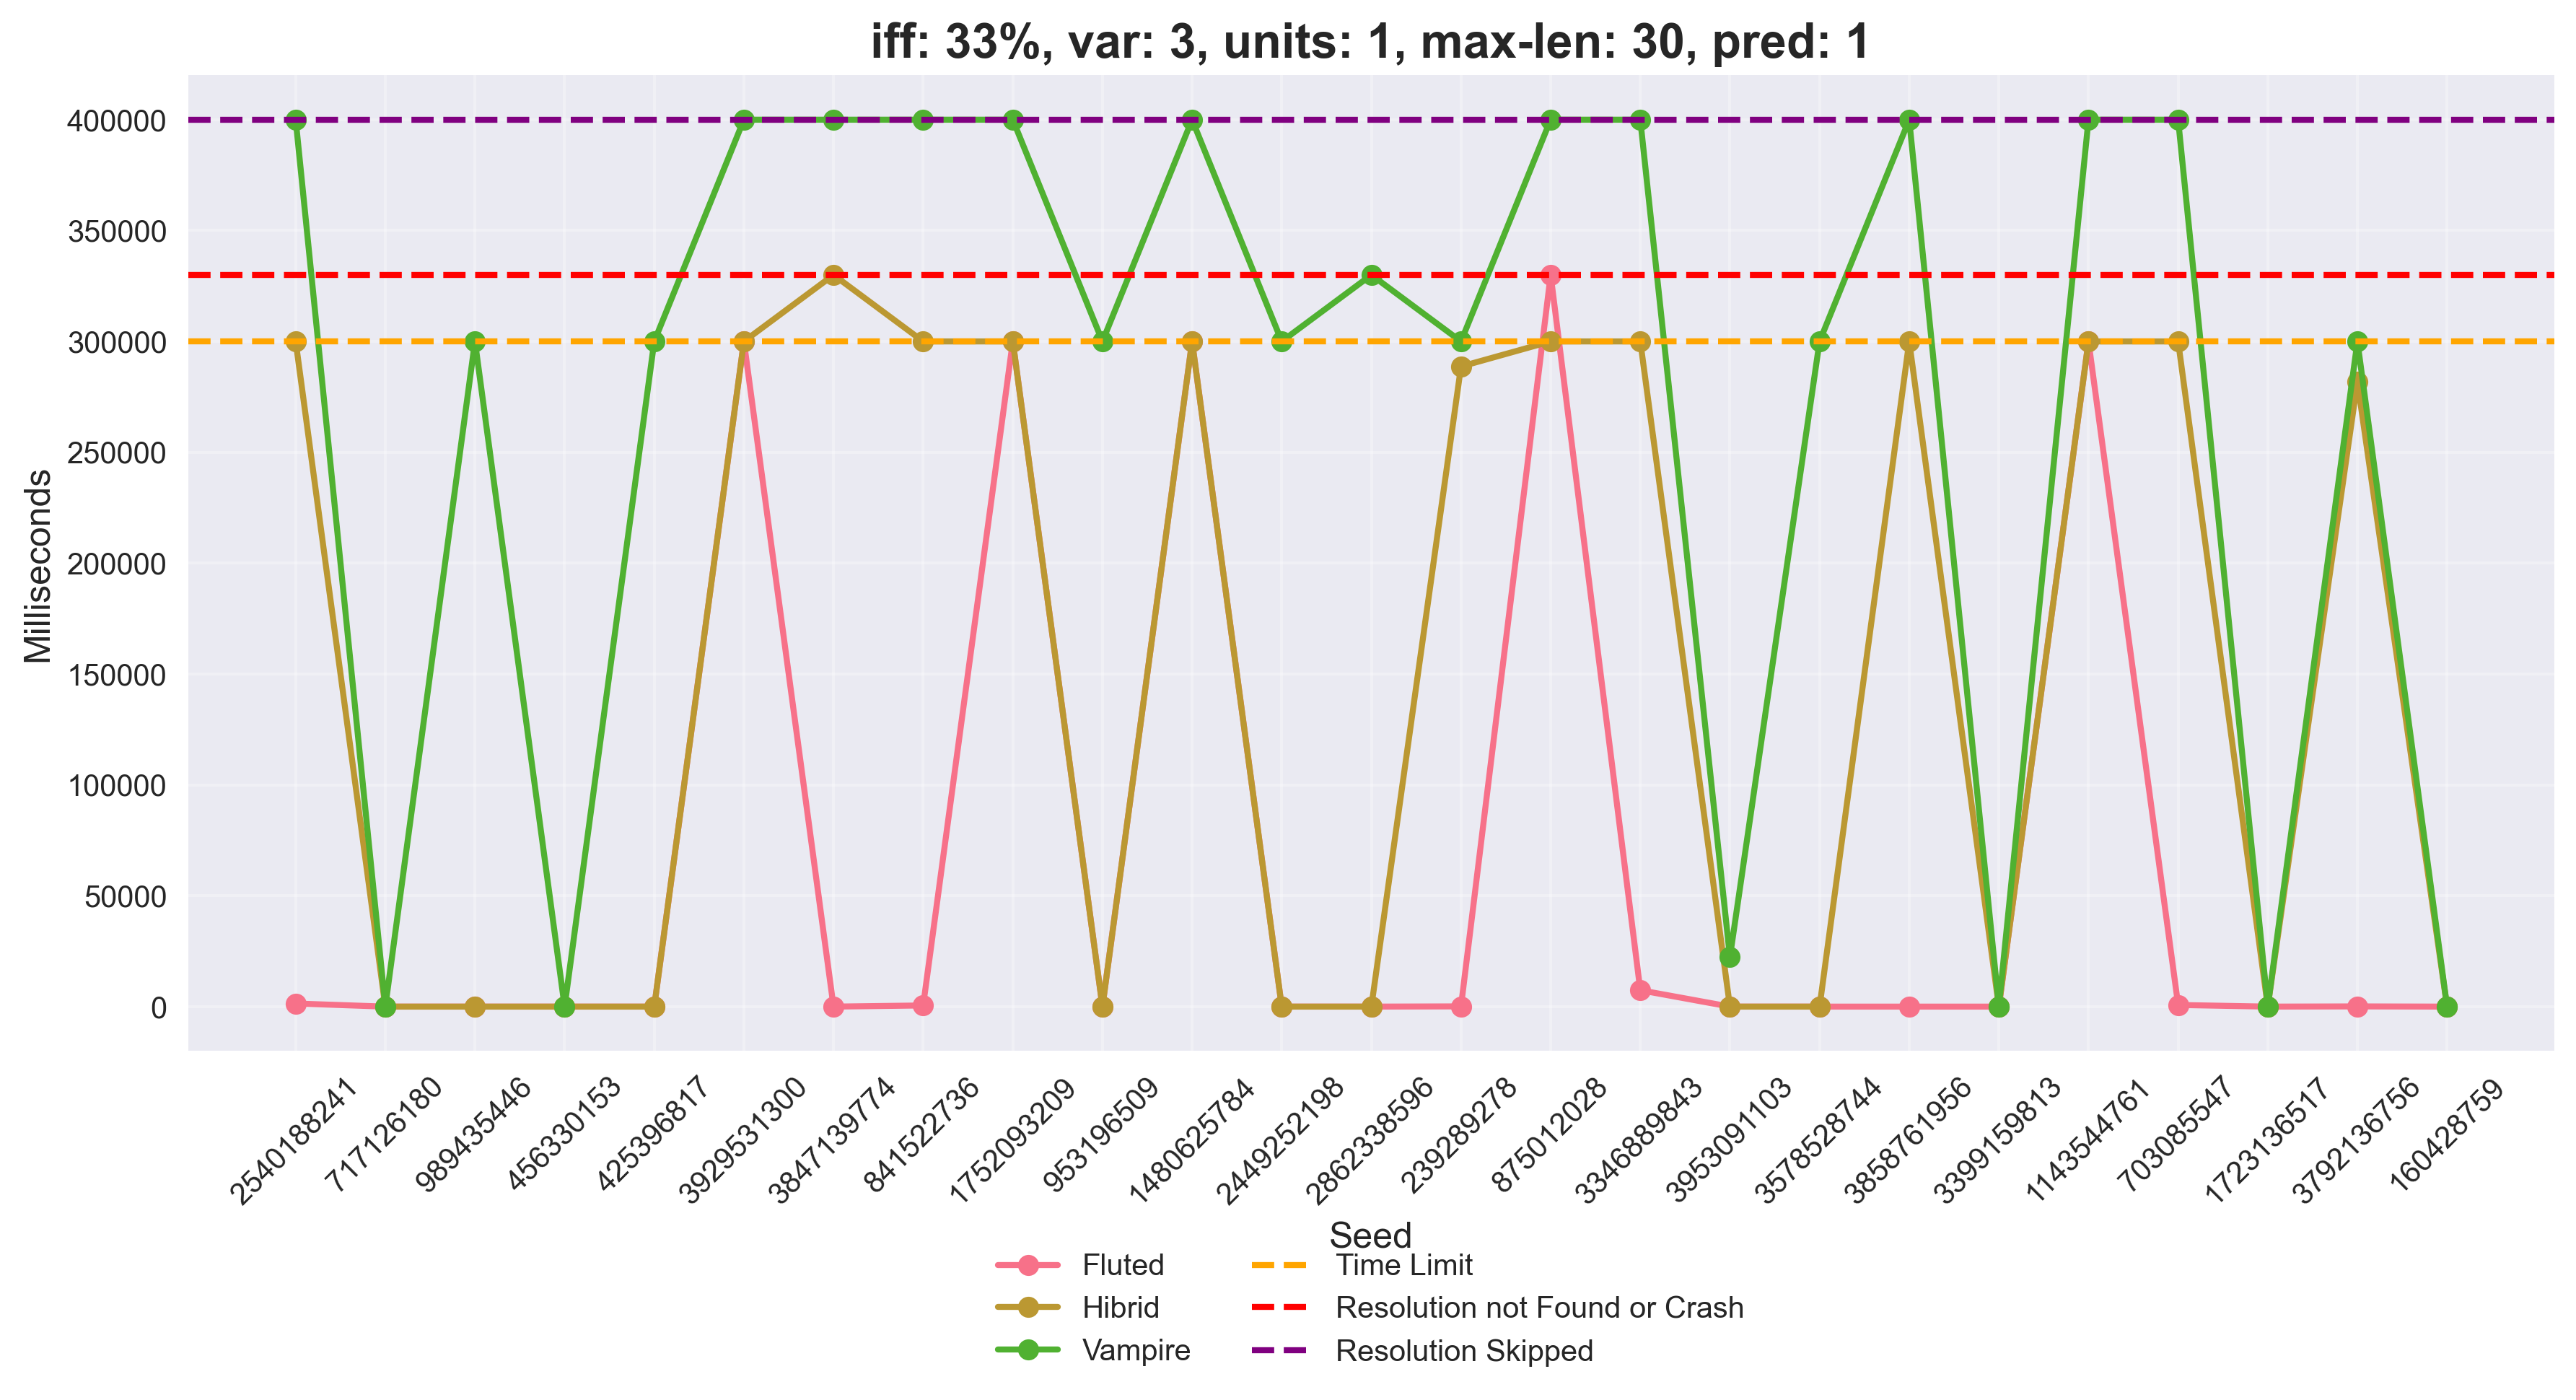
\includegraphics[width=\textwidth]{7-generated-benchmarking/singles/res-16_linee_normal.png}
\end{figure}
\begin{figure}[H]
    \centering
    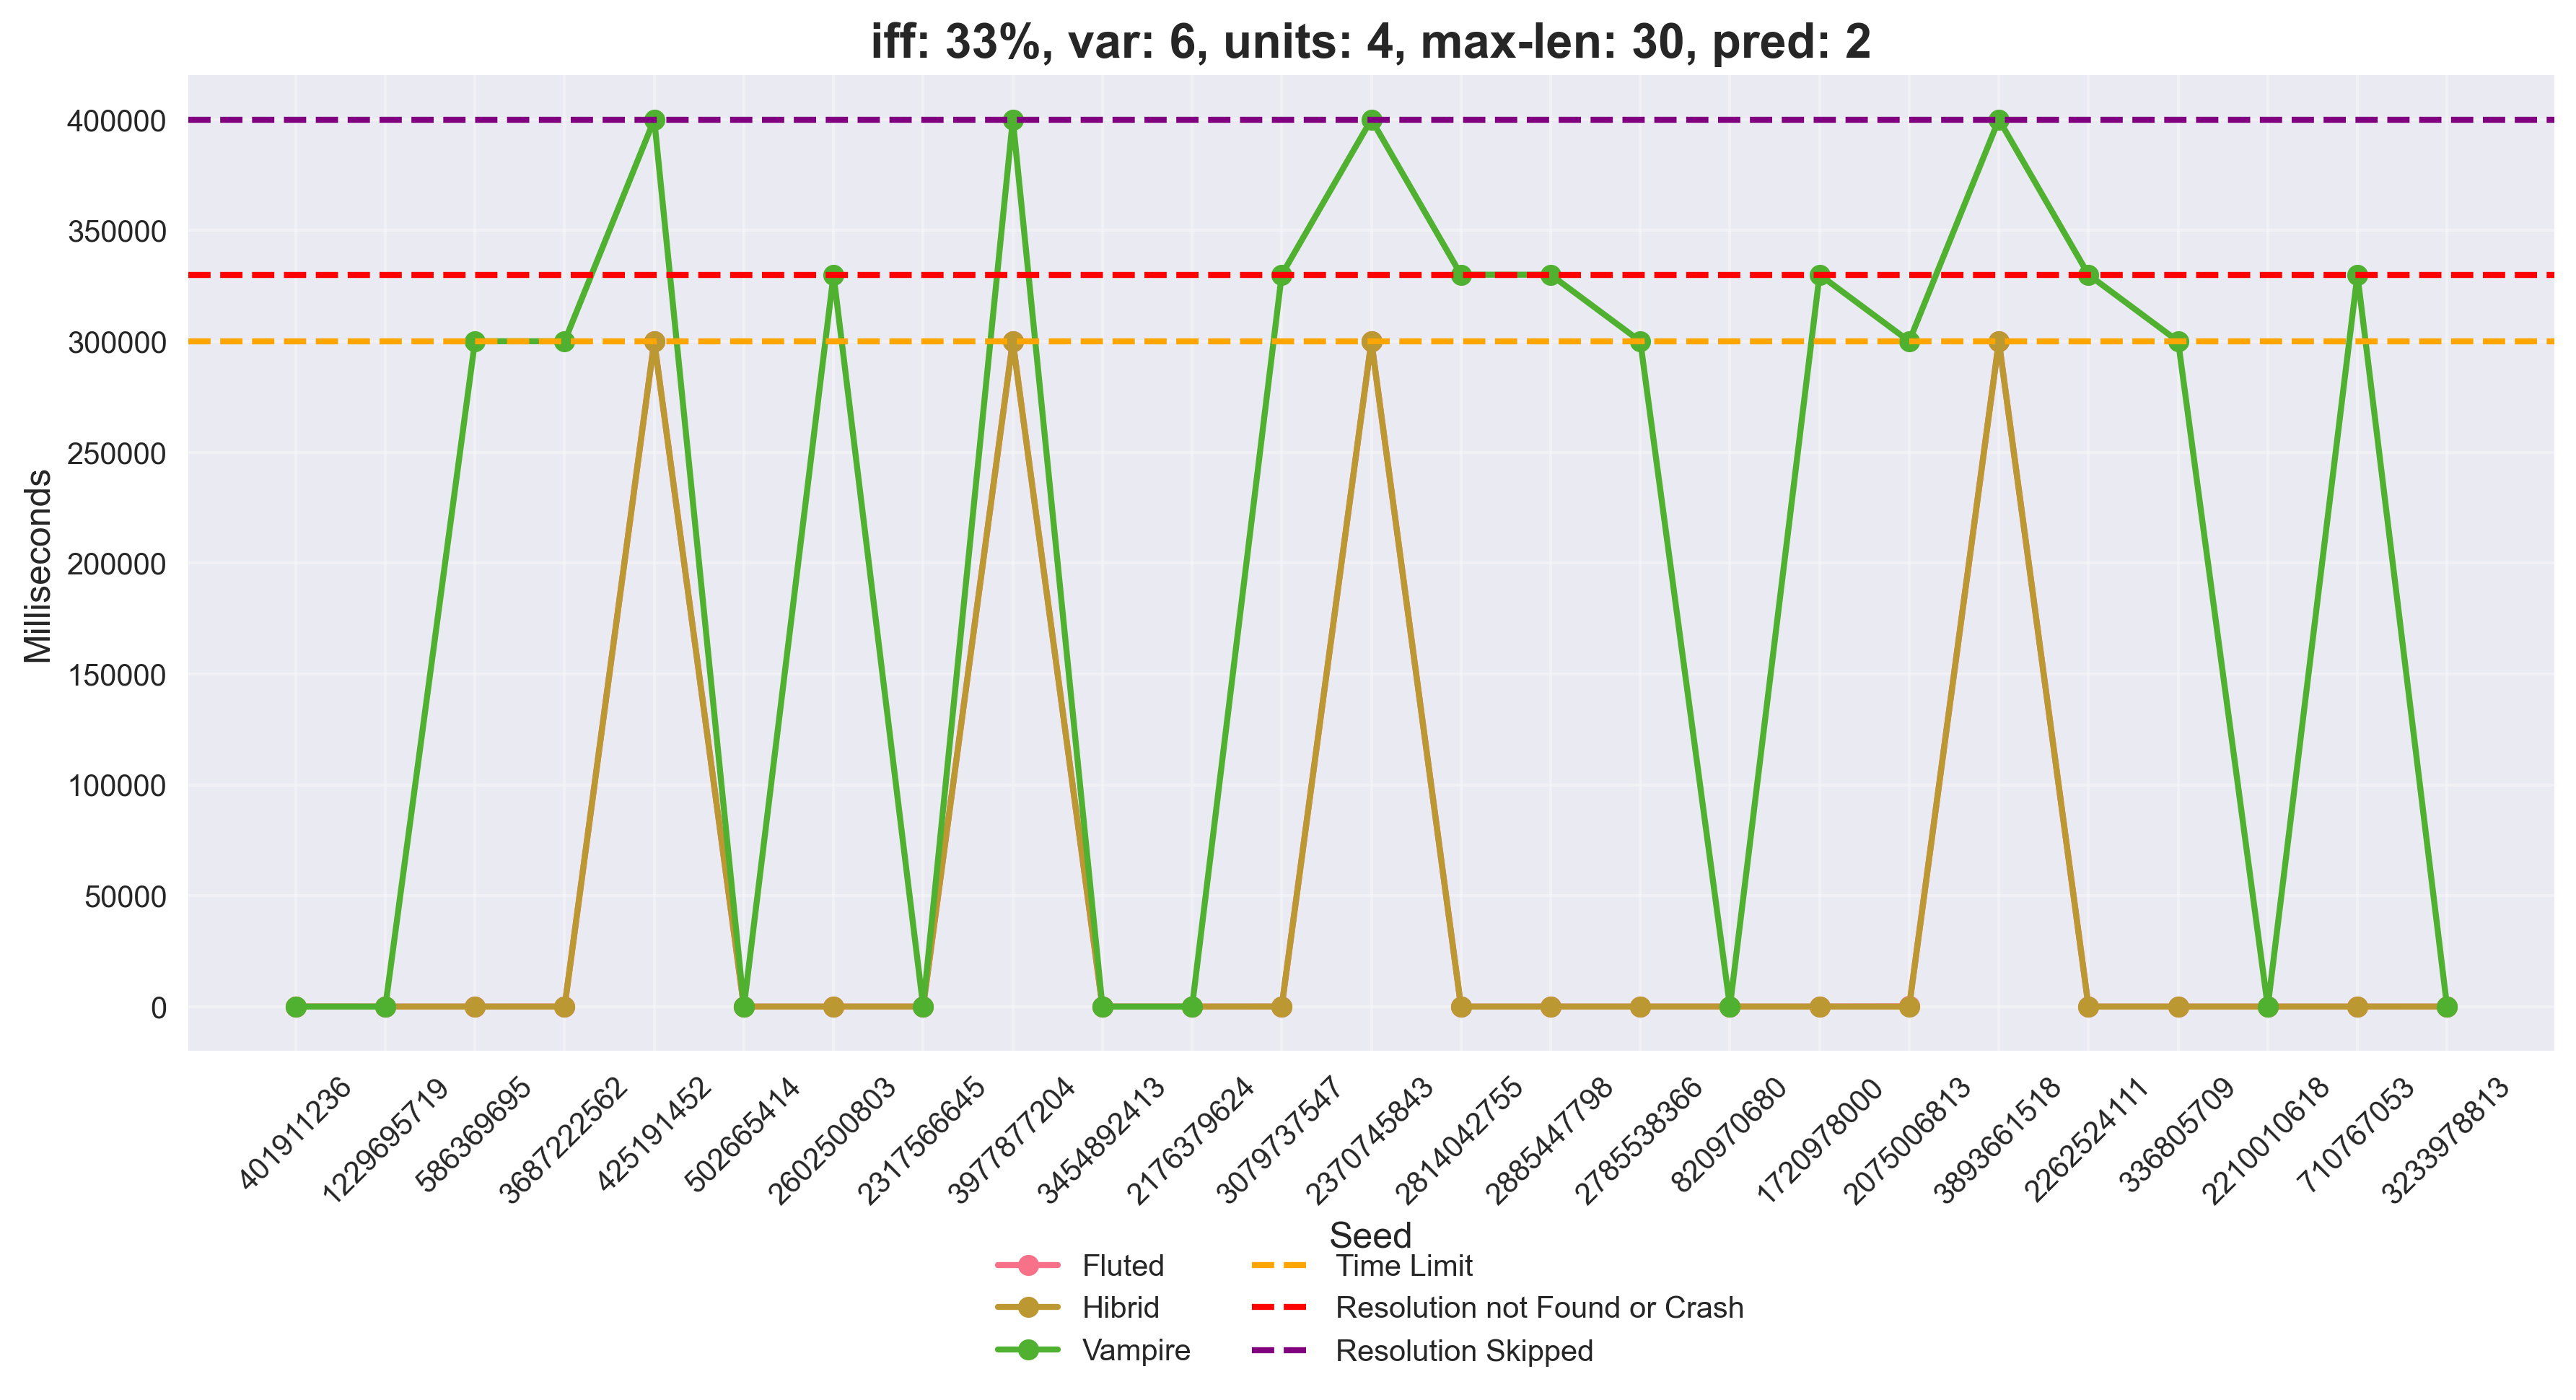
\includegraphics[width=\textwidth]{7-generated-benchmarking/singles/res-37_linee_normal.png}
\end{figure}
\begin{figure}[H]
    \centering
    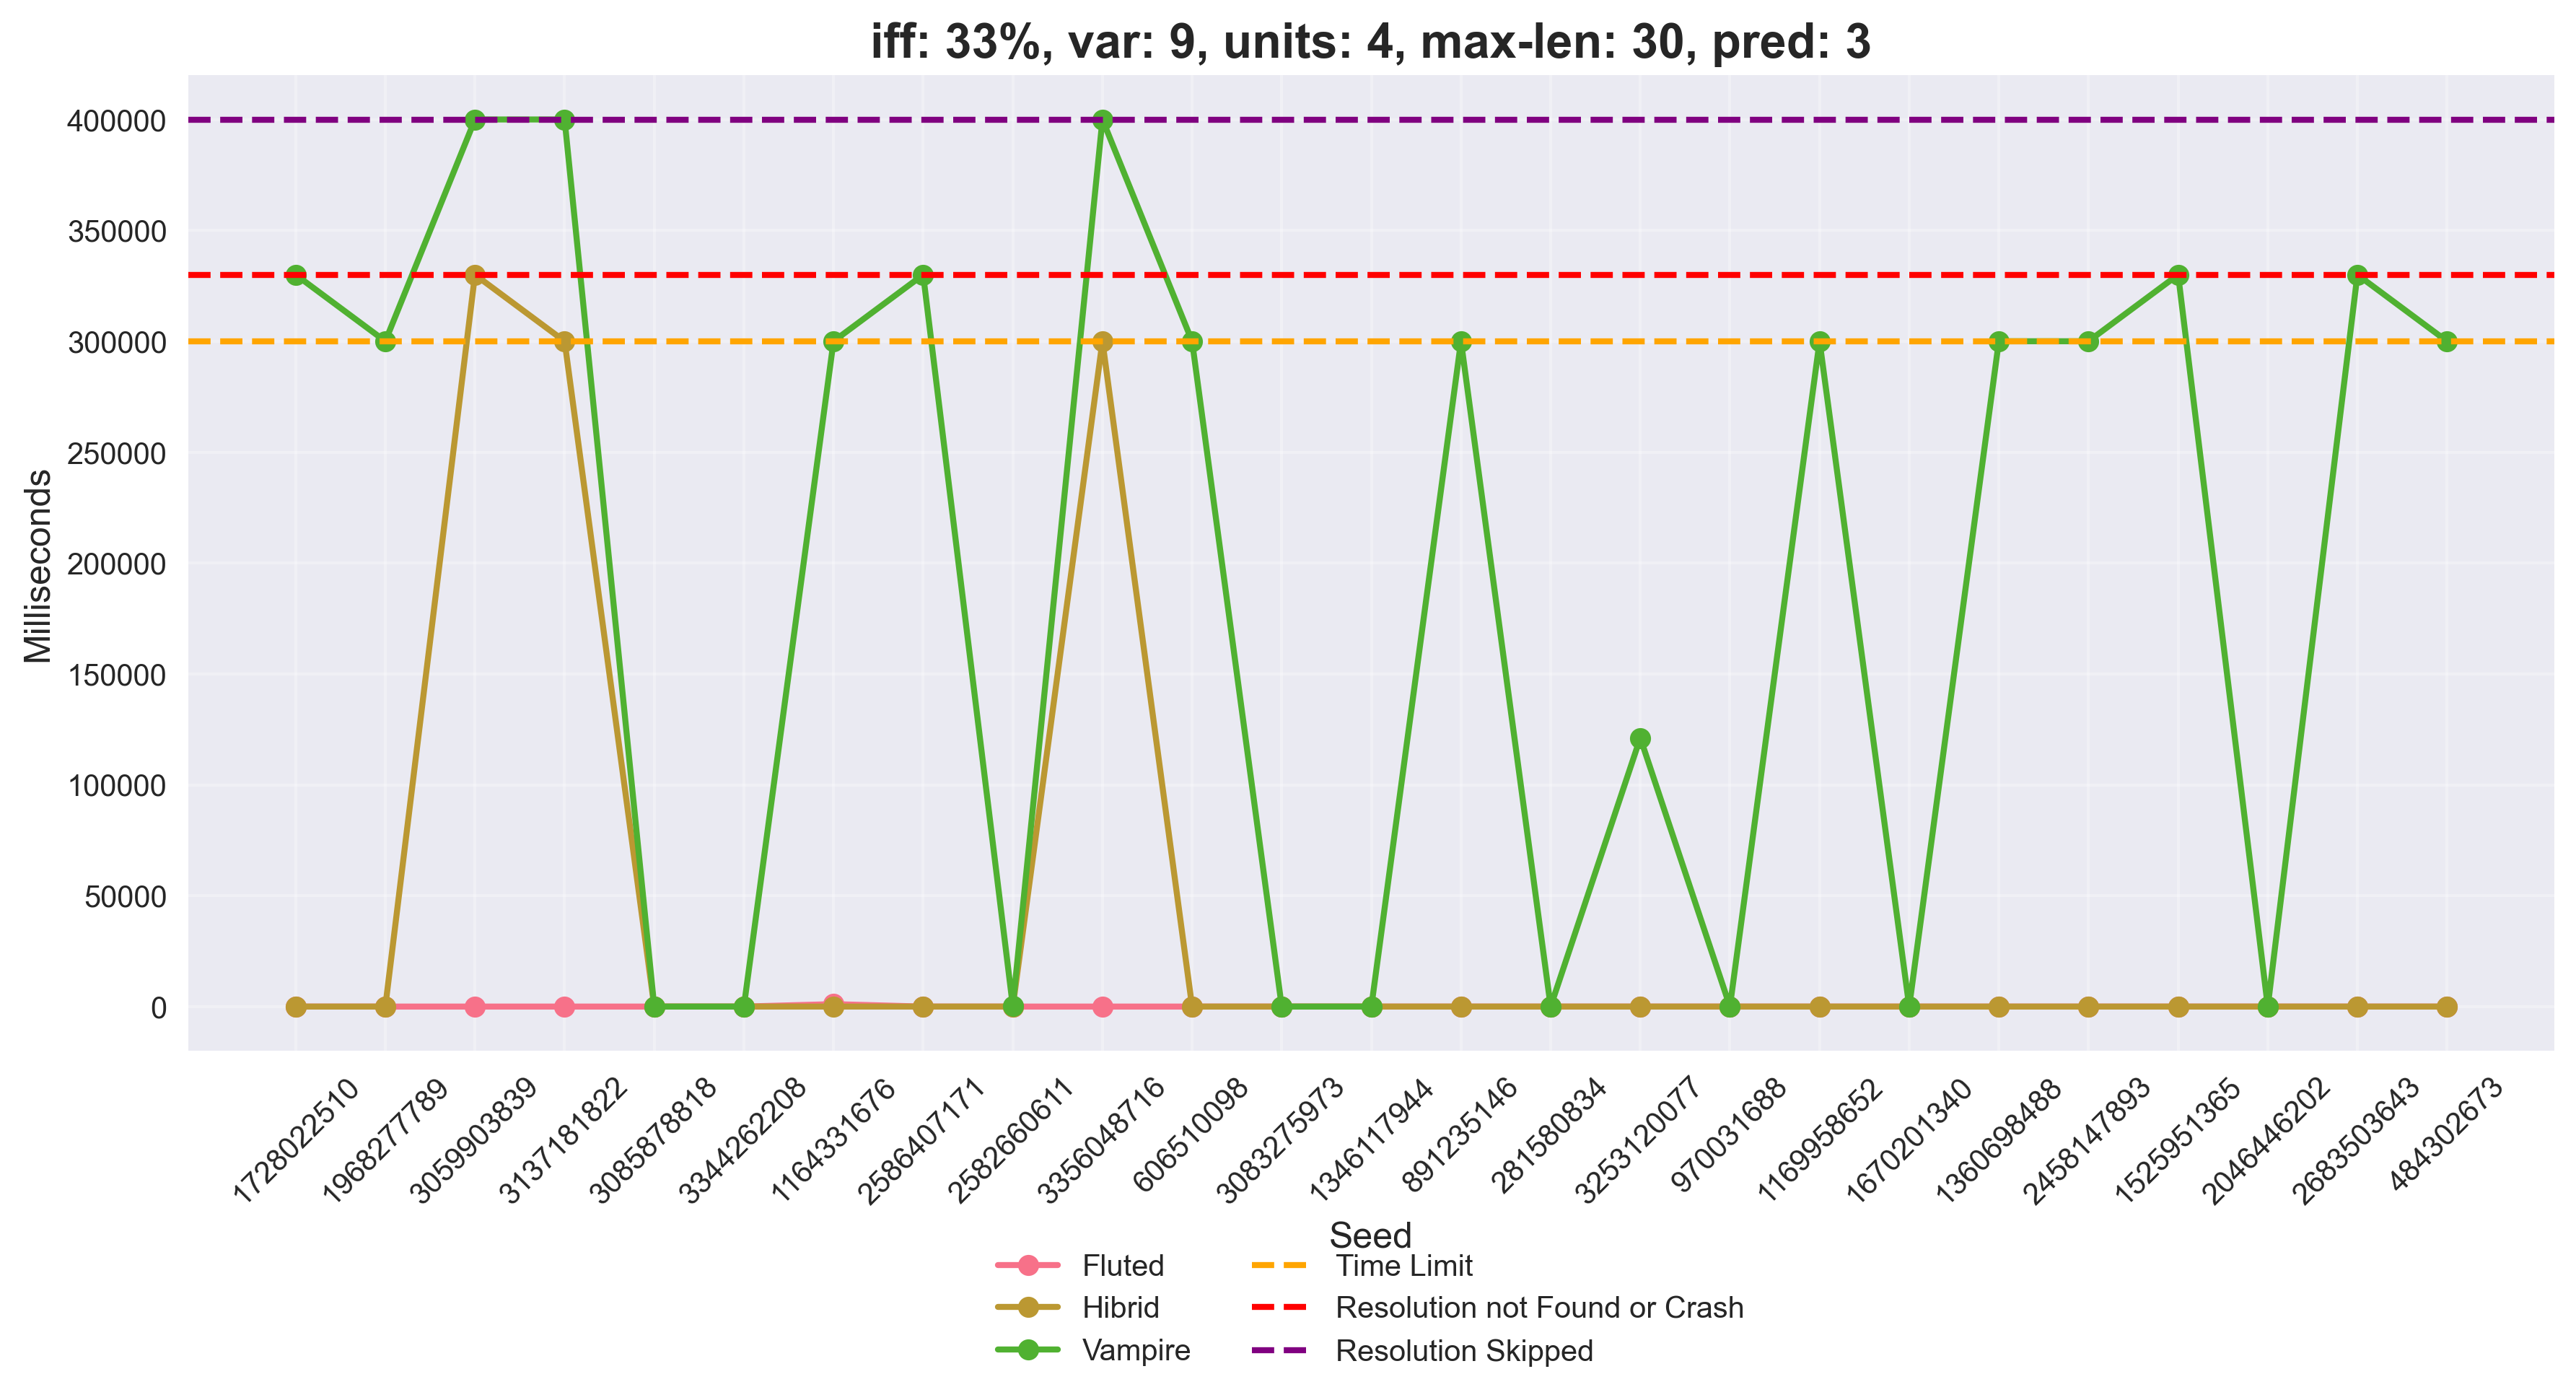
\includegraphics[width=\textwidth]{7-generated-benchmarking/singles/res-57_linee_normal.png}
\end{figure}

These charts do not reveal much more than the CNF problems from TPTP, as the number of problems in each chart is still relatively small.
They, however, confirm the polarization of the results, with most problems being solved very quickly and a few taking a long time or timing out.
To get a more comprehensive view of the performance across all generated problems, we turn to aggregated results.
The first family of aggregated charts we present are the ones fixing the number of variables, varying on the encoded triple \((\text{\code{_predNum}}, \text{\code{_maxLen}}, \text{\code{_unitsNum}})\).
To better highlight the differences between vampire and the other two modes (hybrid and fluted), we decided to provide two versions of each chart: one with a logarithmic scale including vampire mode, for highlighting the differences from the other two modes, and one with a normal scale excluding vampire mode, to emphasize the differences between hybrid and fluted modes.
\begin{figure}[H]
  \centering
  \begin{minipage}{1\textwidth}
    \centering
    \includegraphics[width=\textwidth]{7-generated-benchmarking/aggregated/var-02/res-avg_linee_log.png}
  \end{minipage}
  \hfill
  \begin{minipage}{1\textwidth}
    \centering
    \includegraphics[width=\textwidth]{7-generated-benchmarking/aggregated/var-02/res-avg_linee_normal.png}
  \end{minipage}
  \caption{Aggregated results for generated problems with \code{_maxArity} = 2.}\label{fig:agg-var2}
\end{figure}

\begin{figure}[H]
  \centering
  \begin{minipage}{\textwidth}
    \centering
    \includegraphics[width=\textwidth]{7-generated-benchmarking/aggregated/var-07/res-avg_linee_log.png}
  \end{minipage}
  \hfill
  \begin{minipage}{\textwidth}
    \centering
    \includegraphics[width=\textwidth]{7-generated-benchmarking/aggregated/var-07/res-avg_linee_normal.png}
  \end{minipage}
  \caption{Aggregated results for generated problems with \code{_maxArity} = 7.}\label{fig:agg-var7}
\end{figure}
Full displays of all the aggregated charts for fixed \code{_maxArity} values from \(2\) to \(9\) can be found in the Appendix~\ref{app:charts-by-maxlen-unitsnum}.

As it is possible to see, all charts show a similar pattern, with remarkable spikes around the intervals \((13+20k, 17+20k), k \in \mathbb{N}\) of the lexicographic encoding.
The regularity of these spikes suggests that they are related to specific combinations of the parameters. In particular, seeing that the spikes occur every \(20\) units on the x-axis, it is likely that they are independent of \code{_predNum}, which changes every \(20\) units, and are instead related to \code{_maxLen} and \code{_unitsNum}, which change more frequently.
Analysing the encoding of the parameters, we can see that the spikes correspond to combinations where \code{_maxLen} is close to its maximum and \code{_unitsNum} is close to its minimum.

\begin{figure}[H]
  \centering
  \begin{minipage}{0.8\textwidth}
    \centering
    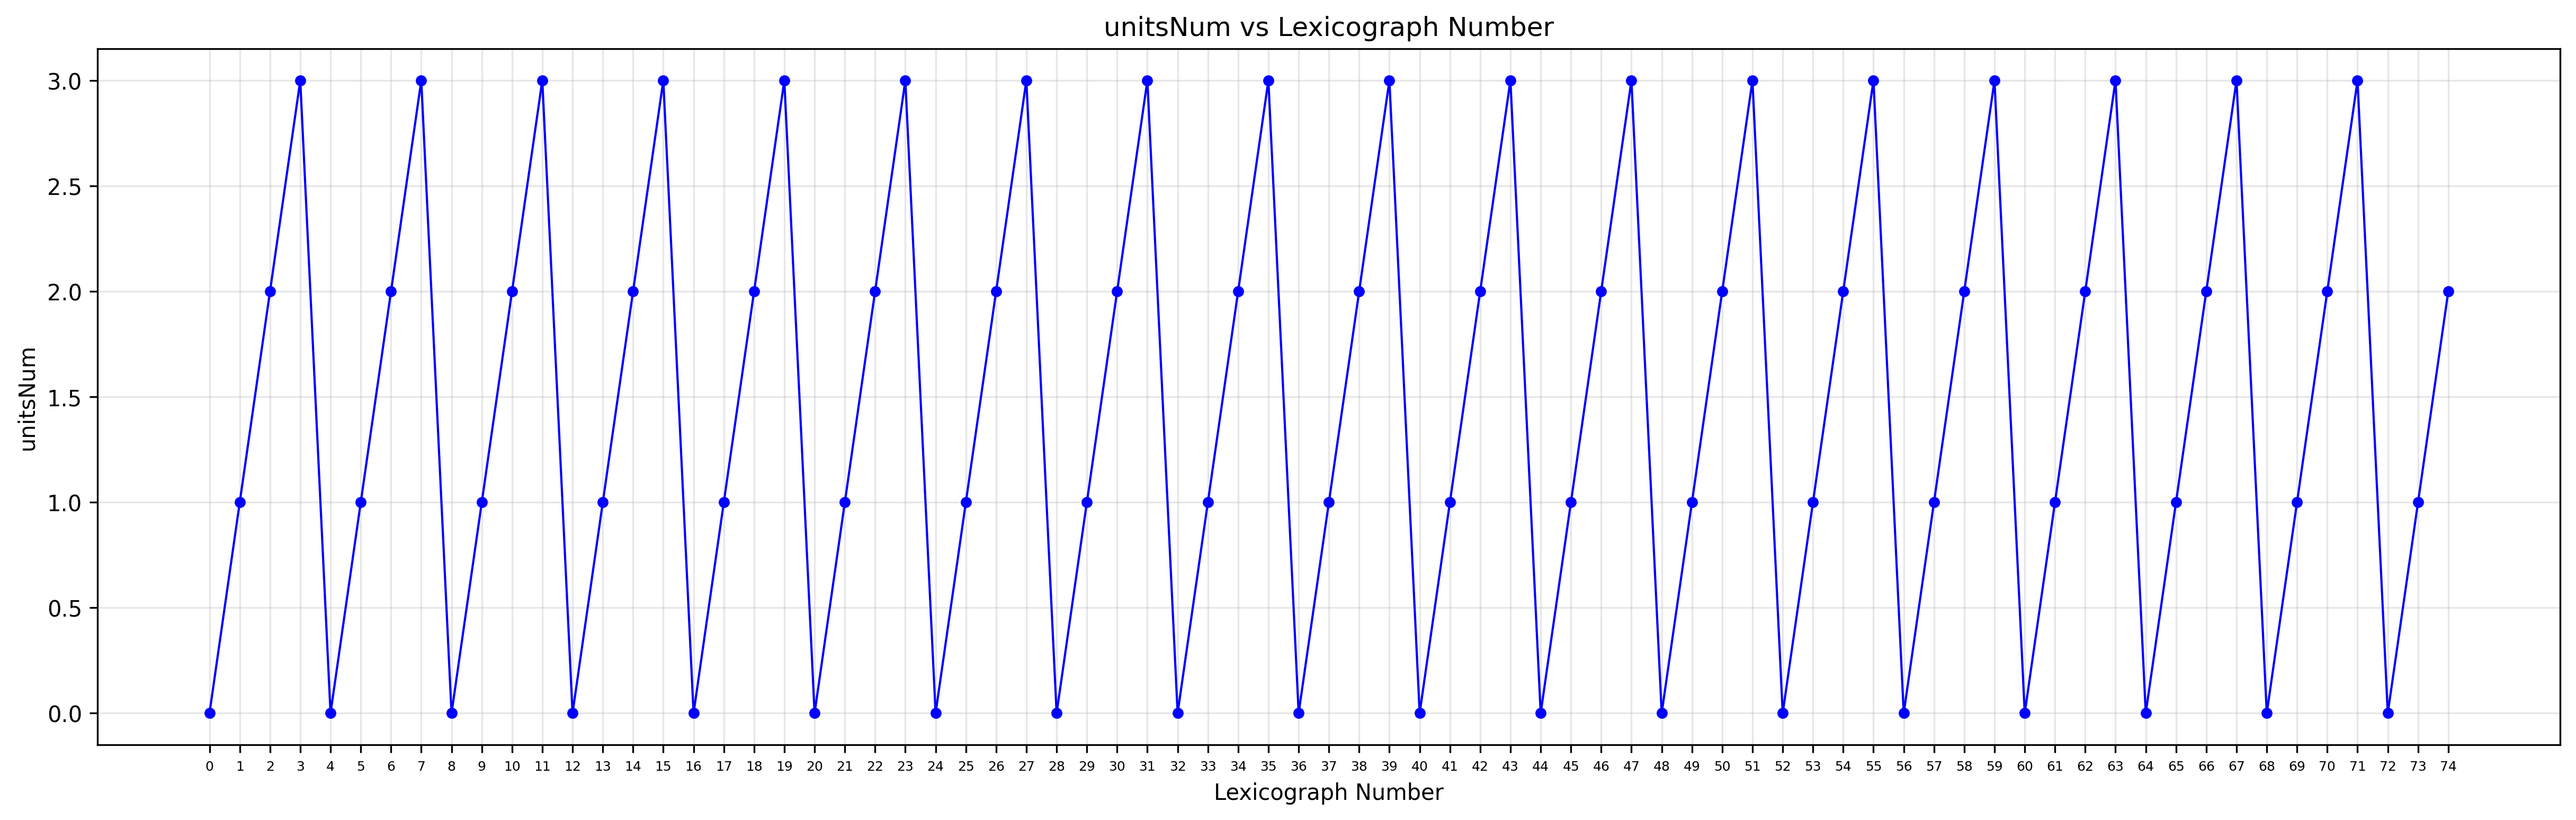
\includegraphics[width=\textwidth]{7-generated-benchmarking/aggregated/unitsNum_plot.png}
    \caption{Units number progression}\label{fig:unitsnum-progression}
  \end{minipage}
  \hfill
  \begin{minipage}{0.8\textwidth}
    \centering
    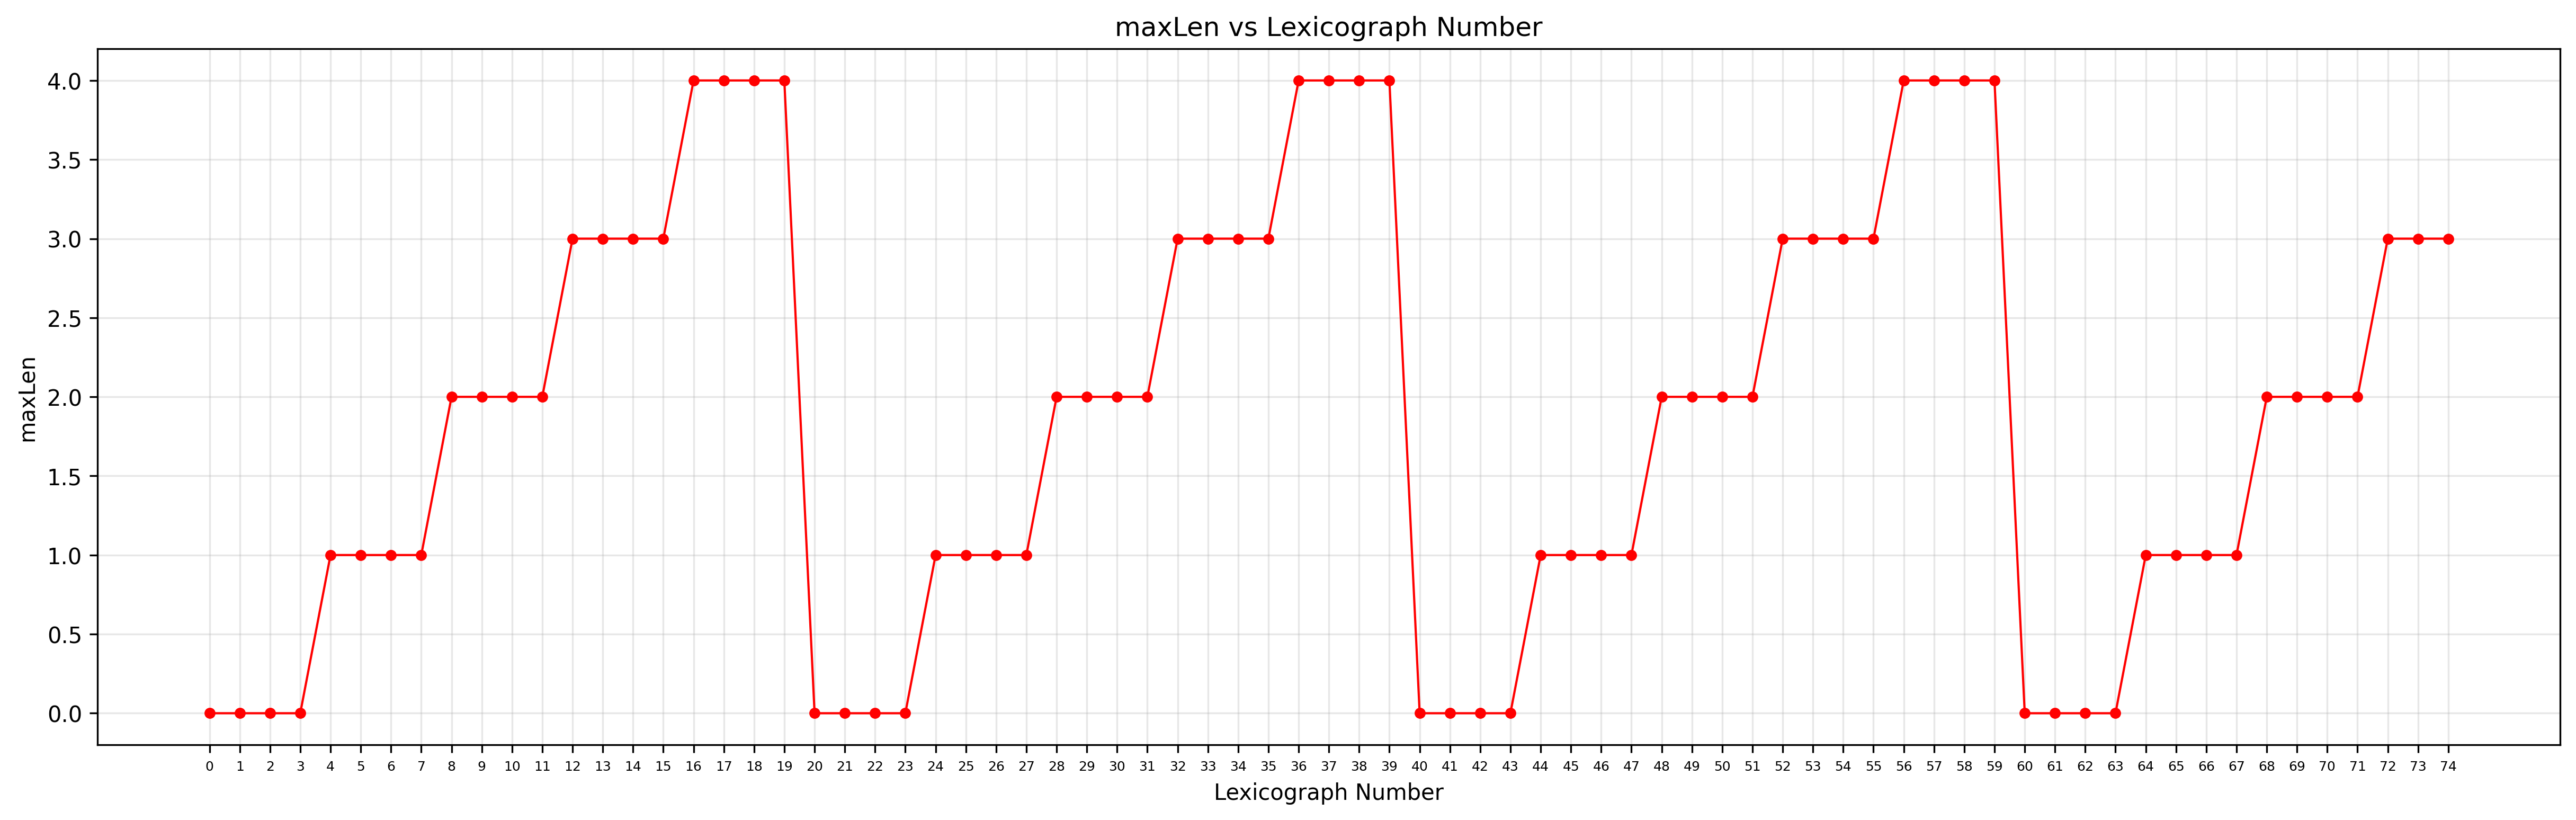
\includegraphics[width=\textwidth]{7-generated-benchmarking/aggregated/maxLenIdx_plot.png}
    \caption{Maximal length progression}\label{fig:maxlen-progression}
  \end{minipage}
\end{figure}
\begin{figure}[H]
  \centering
  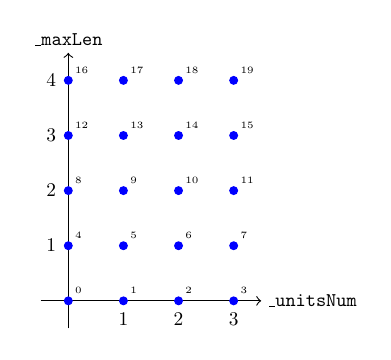
\begin{tikzpicture}[scale=0.7,transform shape]
    % Assi
    \draw[->] (-0.5,0) -- (3.5,0) node[right] {\texttt{\_unitsNum}};
    \draw[->] (0,-0.5) -- (0,4.5) node[above] {\texttt{\_maxLen}};

    % Puntini e label
    \foreach \x in {0,...,3} {
      \foreach \y in {0,...,4} {
        \filldraw[blue] (\x,\y) circle (2pt);
        \node[anchor=south west, font=\tiny] at (\x,\y) {\pgfmathtruncatemacro{\result}{\x+\y*4}\result};
      }
    }

    % Tick labels per x
    \foreach \x in {1,...,3} {
      \node[below] at (\x,-0.1) {\x};
    }

    % Tick labels per y
    \foreach \y in {1,...,4} {
      \node[left] at (-0.1,\y) {\y};
    }
  \end{tikzpicture}
  \caption{Encoding of \code{_maxLen} and \code{_unitsNum} in the lexicographic ordering.}\label{fig:maxlen-unitsnum-encoding}
\end{figure}
This is probably due to the fact that having a high maximum length allows for more complex formulae, while having a low number of units means that there are fewer opportunities for contradictions to be generated, leading to longer resolution times.
A good analogy can be made with natural language texts: a text composed of a few long sentences is generally harder to understand than a text composed of many short sentences, as the latter provides more opportunities for clarification and resolution of ambiguities.
To further investigate this phenomenon, we provided an additional chart that aggregates the results based on \code{_maxLen} and \code{_unitsNum} alone, averaging over all values of \code{_predNum} and \code{_maxArity}.

\begin{figure}[H]
  \centering
  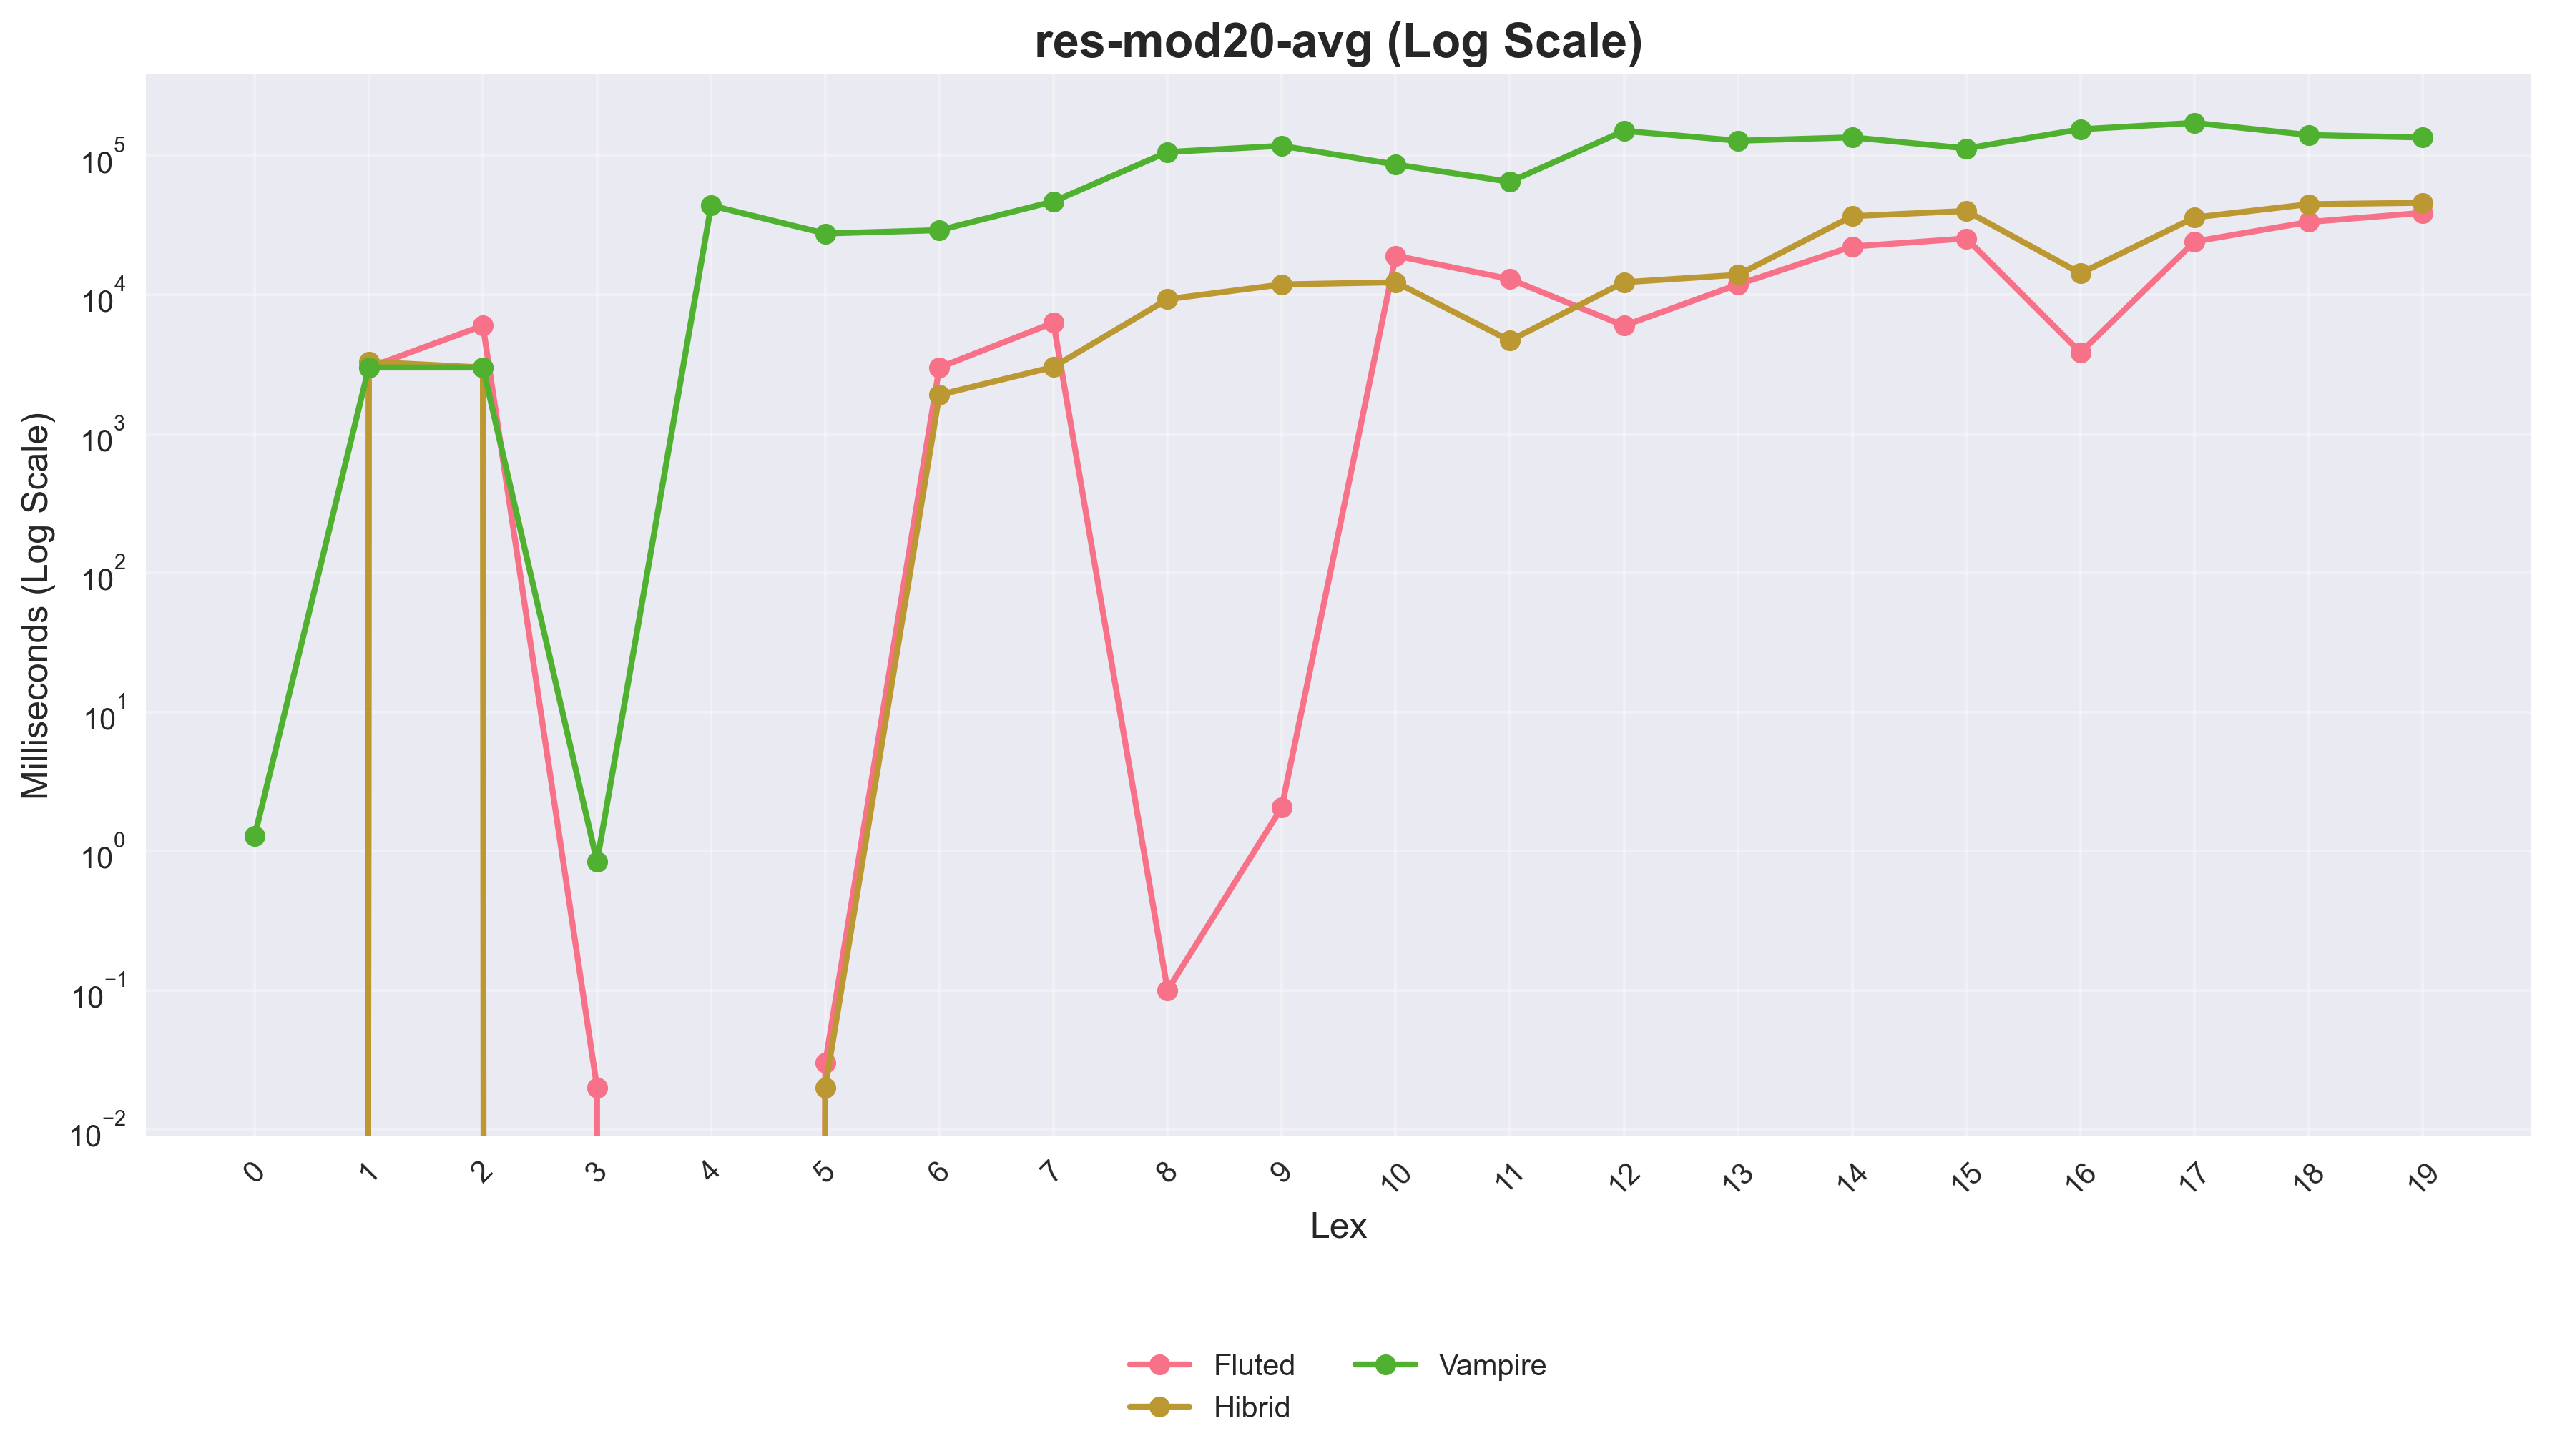
\includegraphics[width=0.8\textwidth]{7-generated-benchmarking/aggregated/res-mod20-avg_linee_log.png}
\end{figure}
\begin{figure}[H]
  \centering
  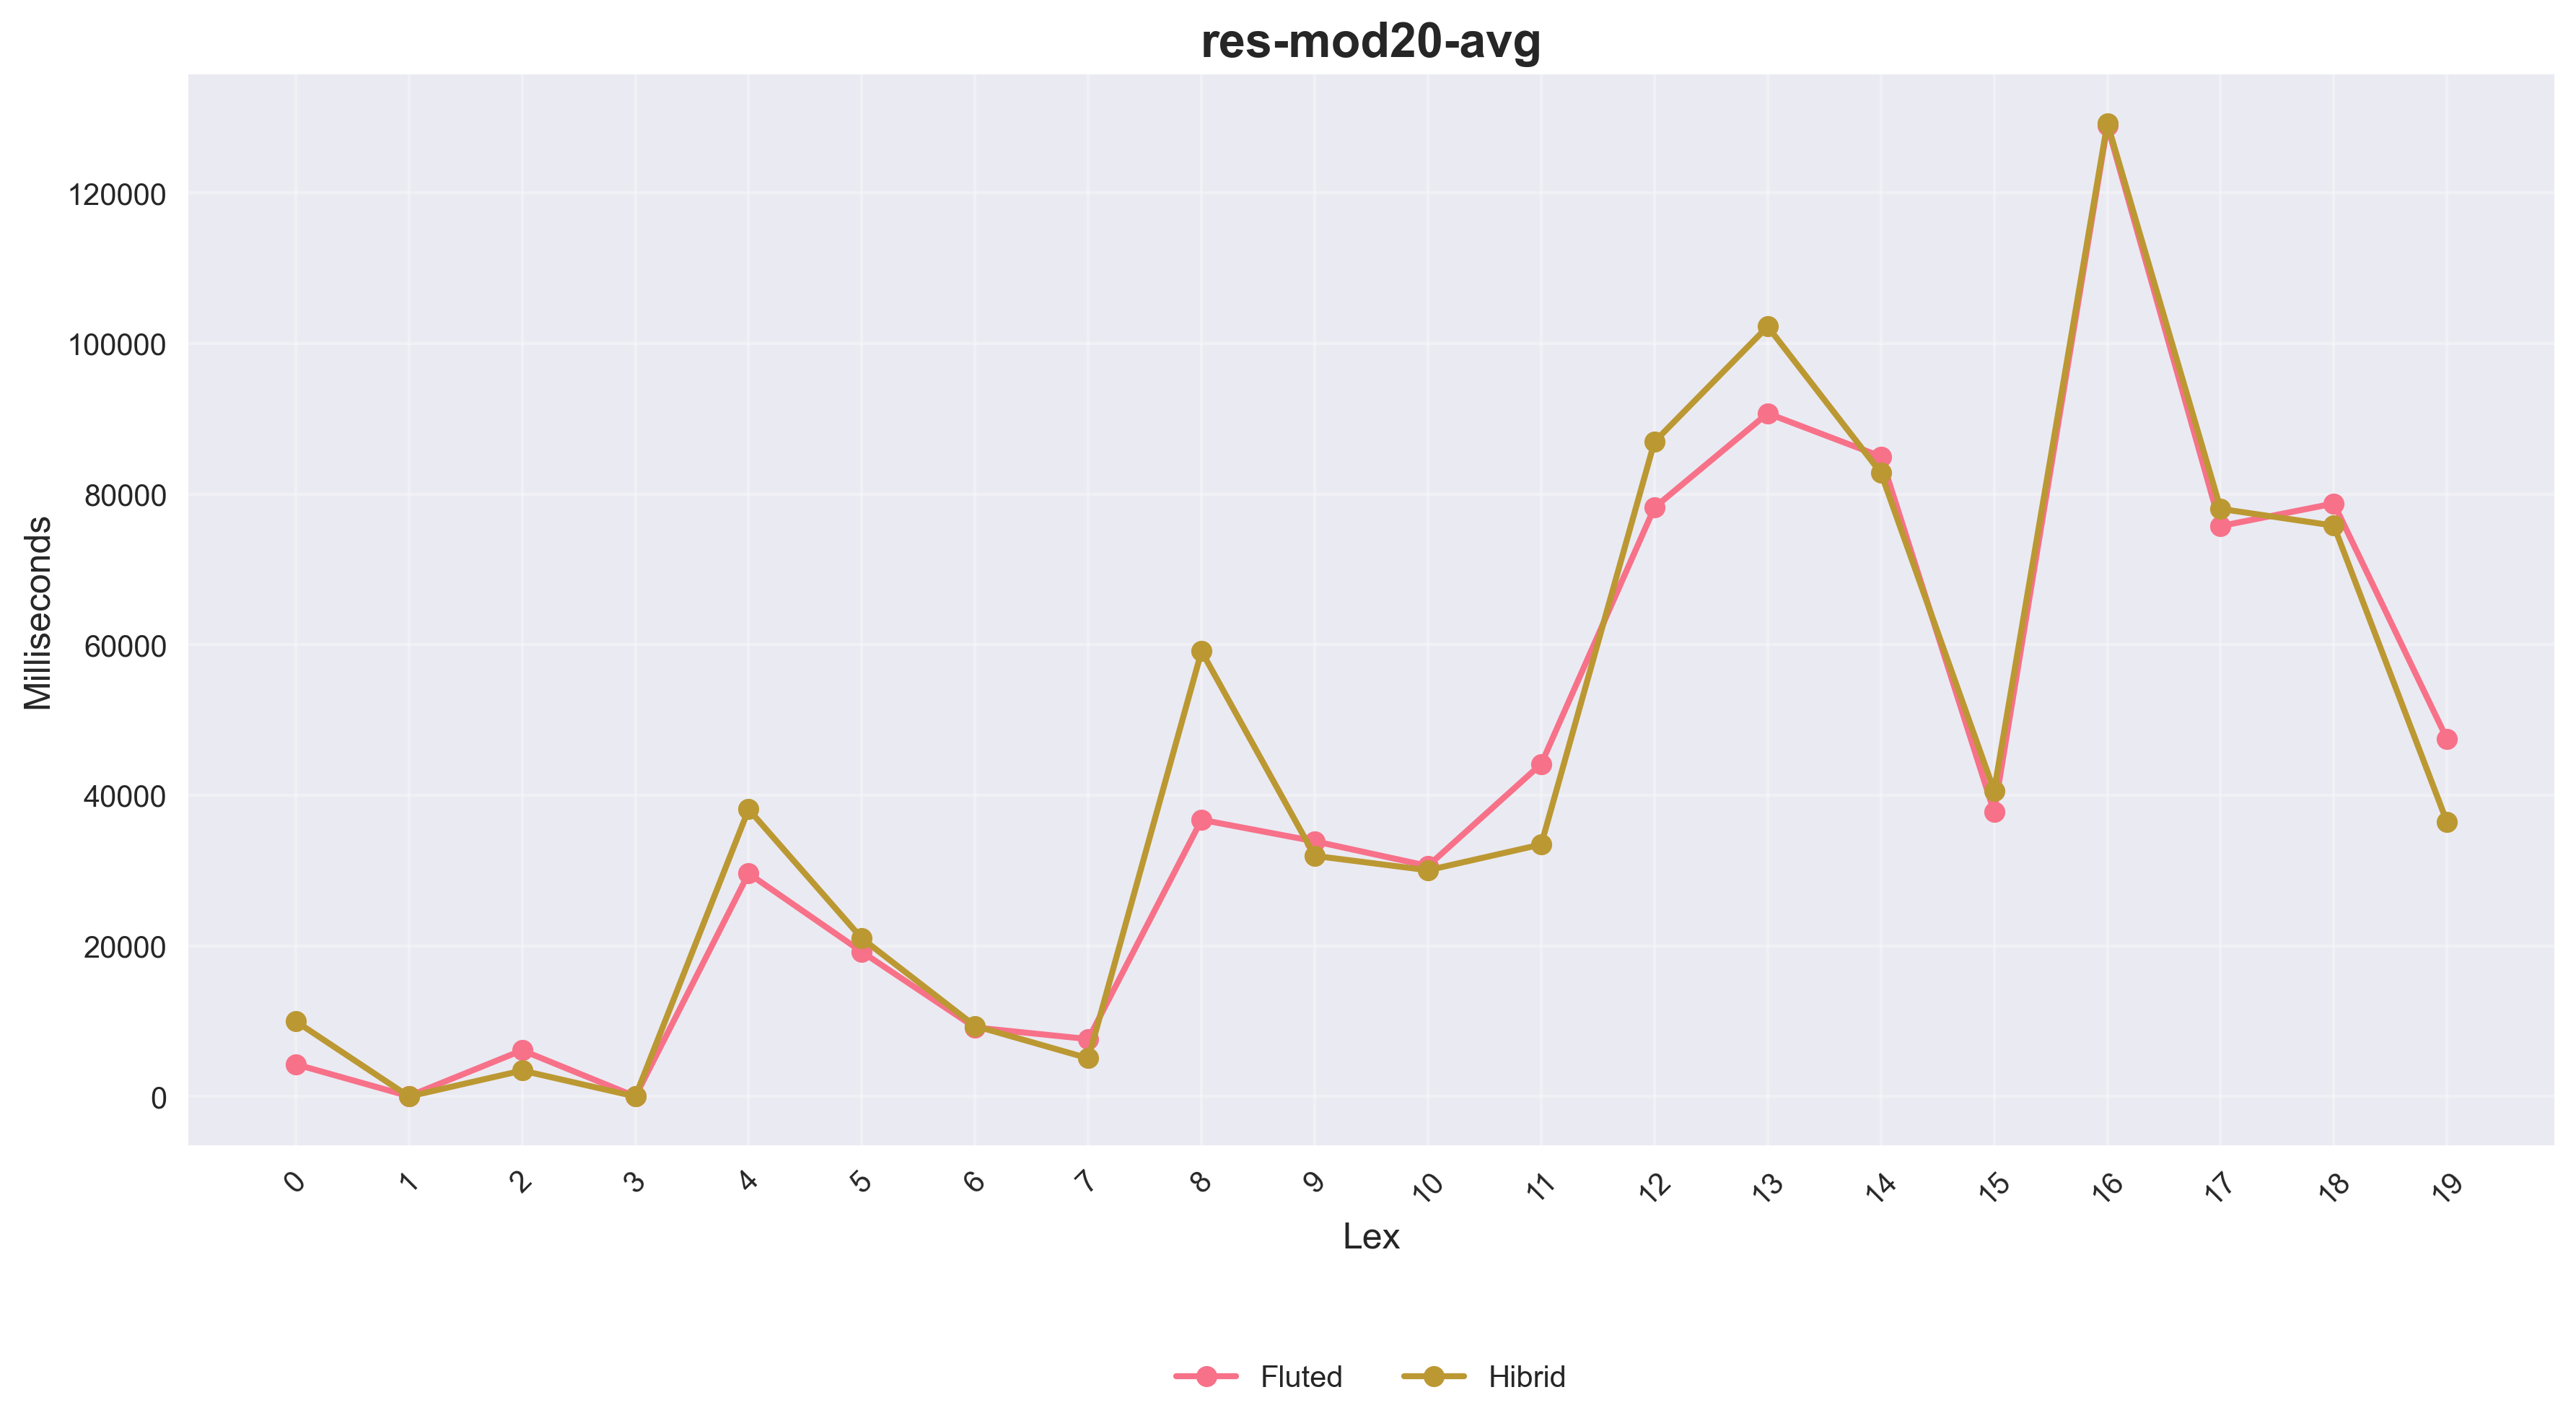
\includegraphics[width=0.8\textwidth]{7-generated-benchmarking/aggregated/res-mod20-avg_linee_normal.png}
  \caption{Aggregated results for generated problems with respect to \code{_maxLen} and \code{_unitsNum}.}\label{fig:agg-maxlen-unitsnum}
\end{figure}
The aggregated versions of the charts with respect to the \code{_predNum} parameter only, with the variable fixed, are provided in Appendix~\ref{app:charts-by-maxlen-unitsnum}.

After this interesting finding, we moved on to analyse the impact of the number of variables on the performance.
To do so, we aggregated the results based on \code{_maxArity} alone, initially fixing the other three parameters.
What follows are examples of such charts, with the full set available in the repository mentioned above.

\begin{figure}[H]
  \centering
  \begin{minipage}{1\textwidth}
    \centering
    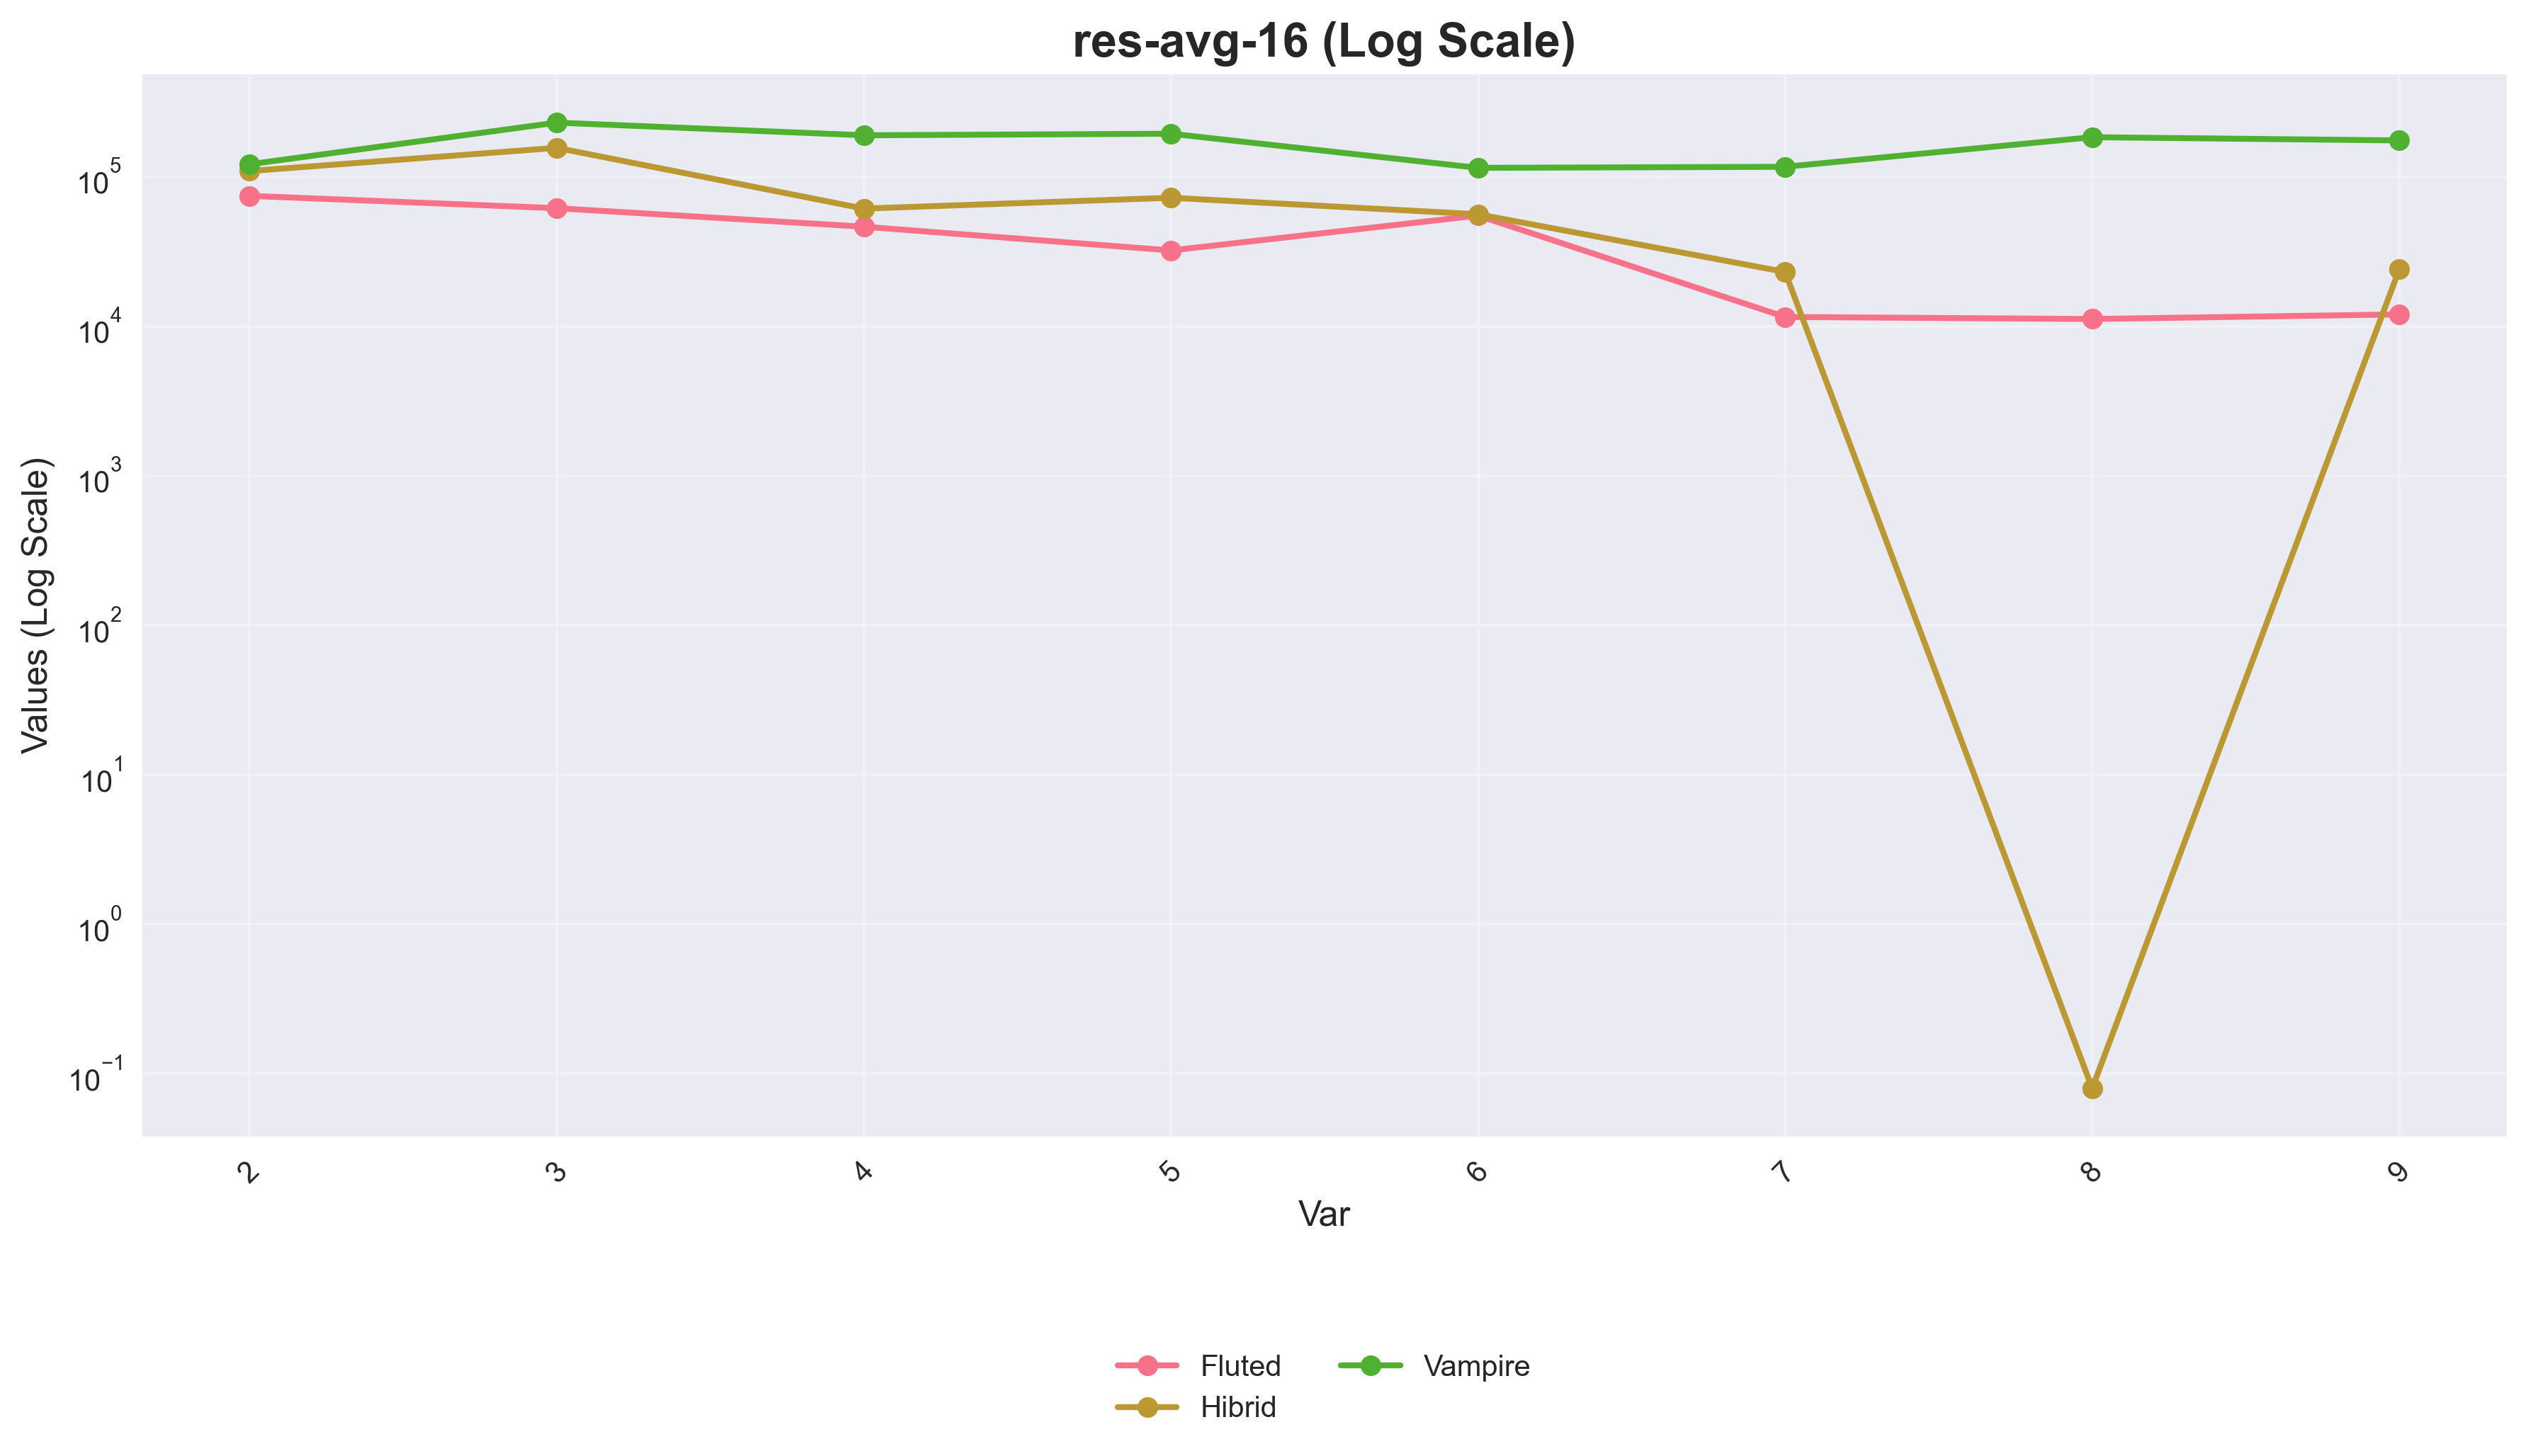
\includegraphics[width=\textwidth]{7-generated-benchmarking/aggregated/res-avg-16_linee_log.png}
  \end{minipage}
  \hfill
  \begin{minipage}{1\textwidth}
    \centering
    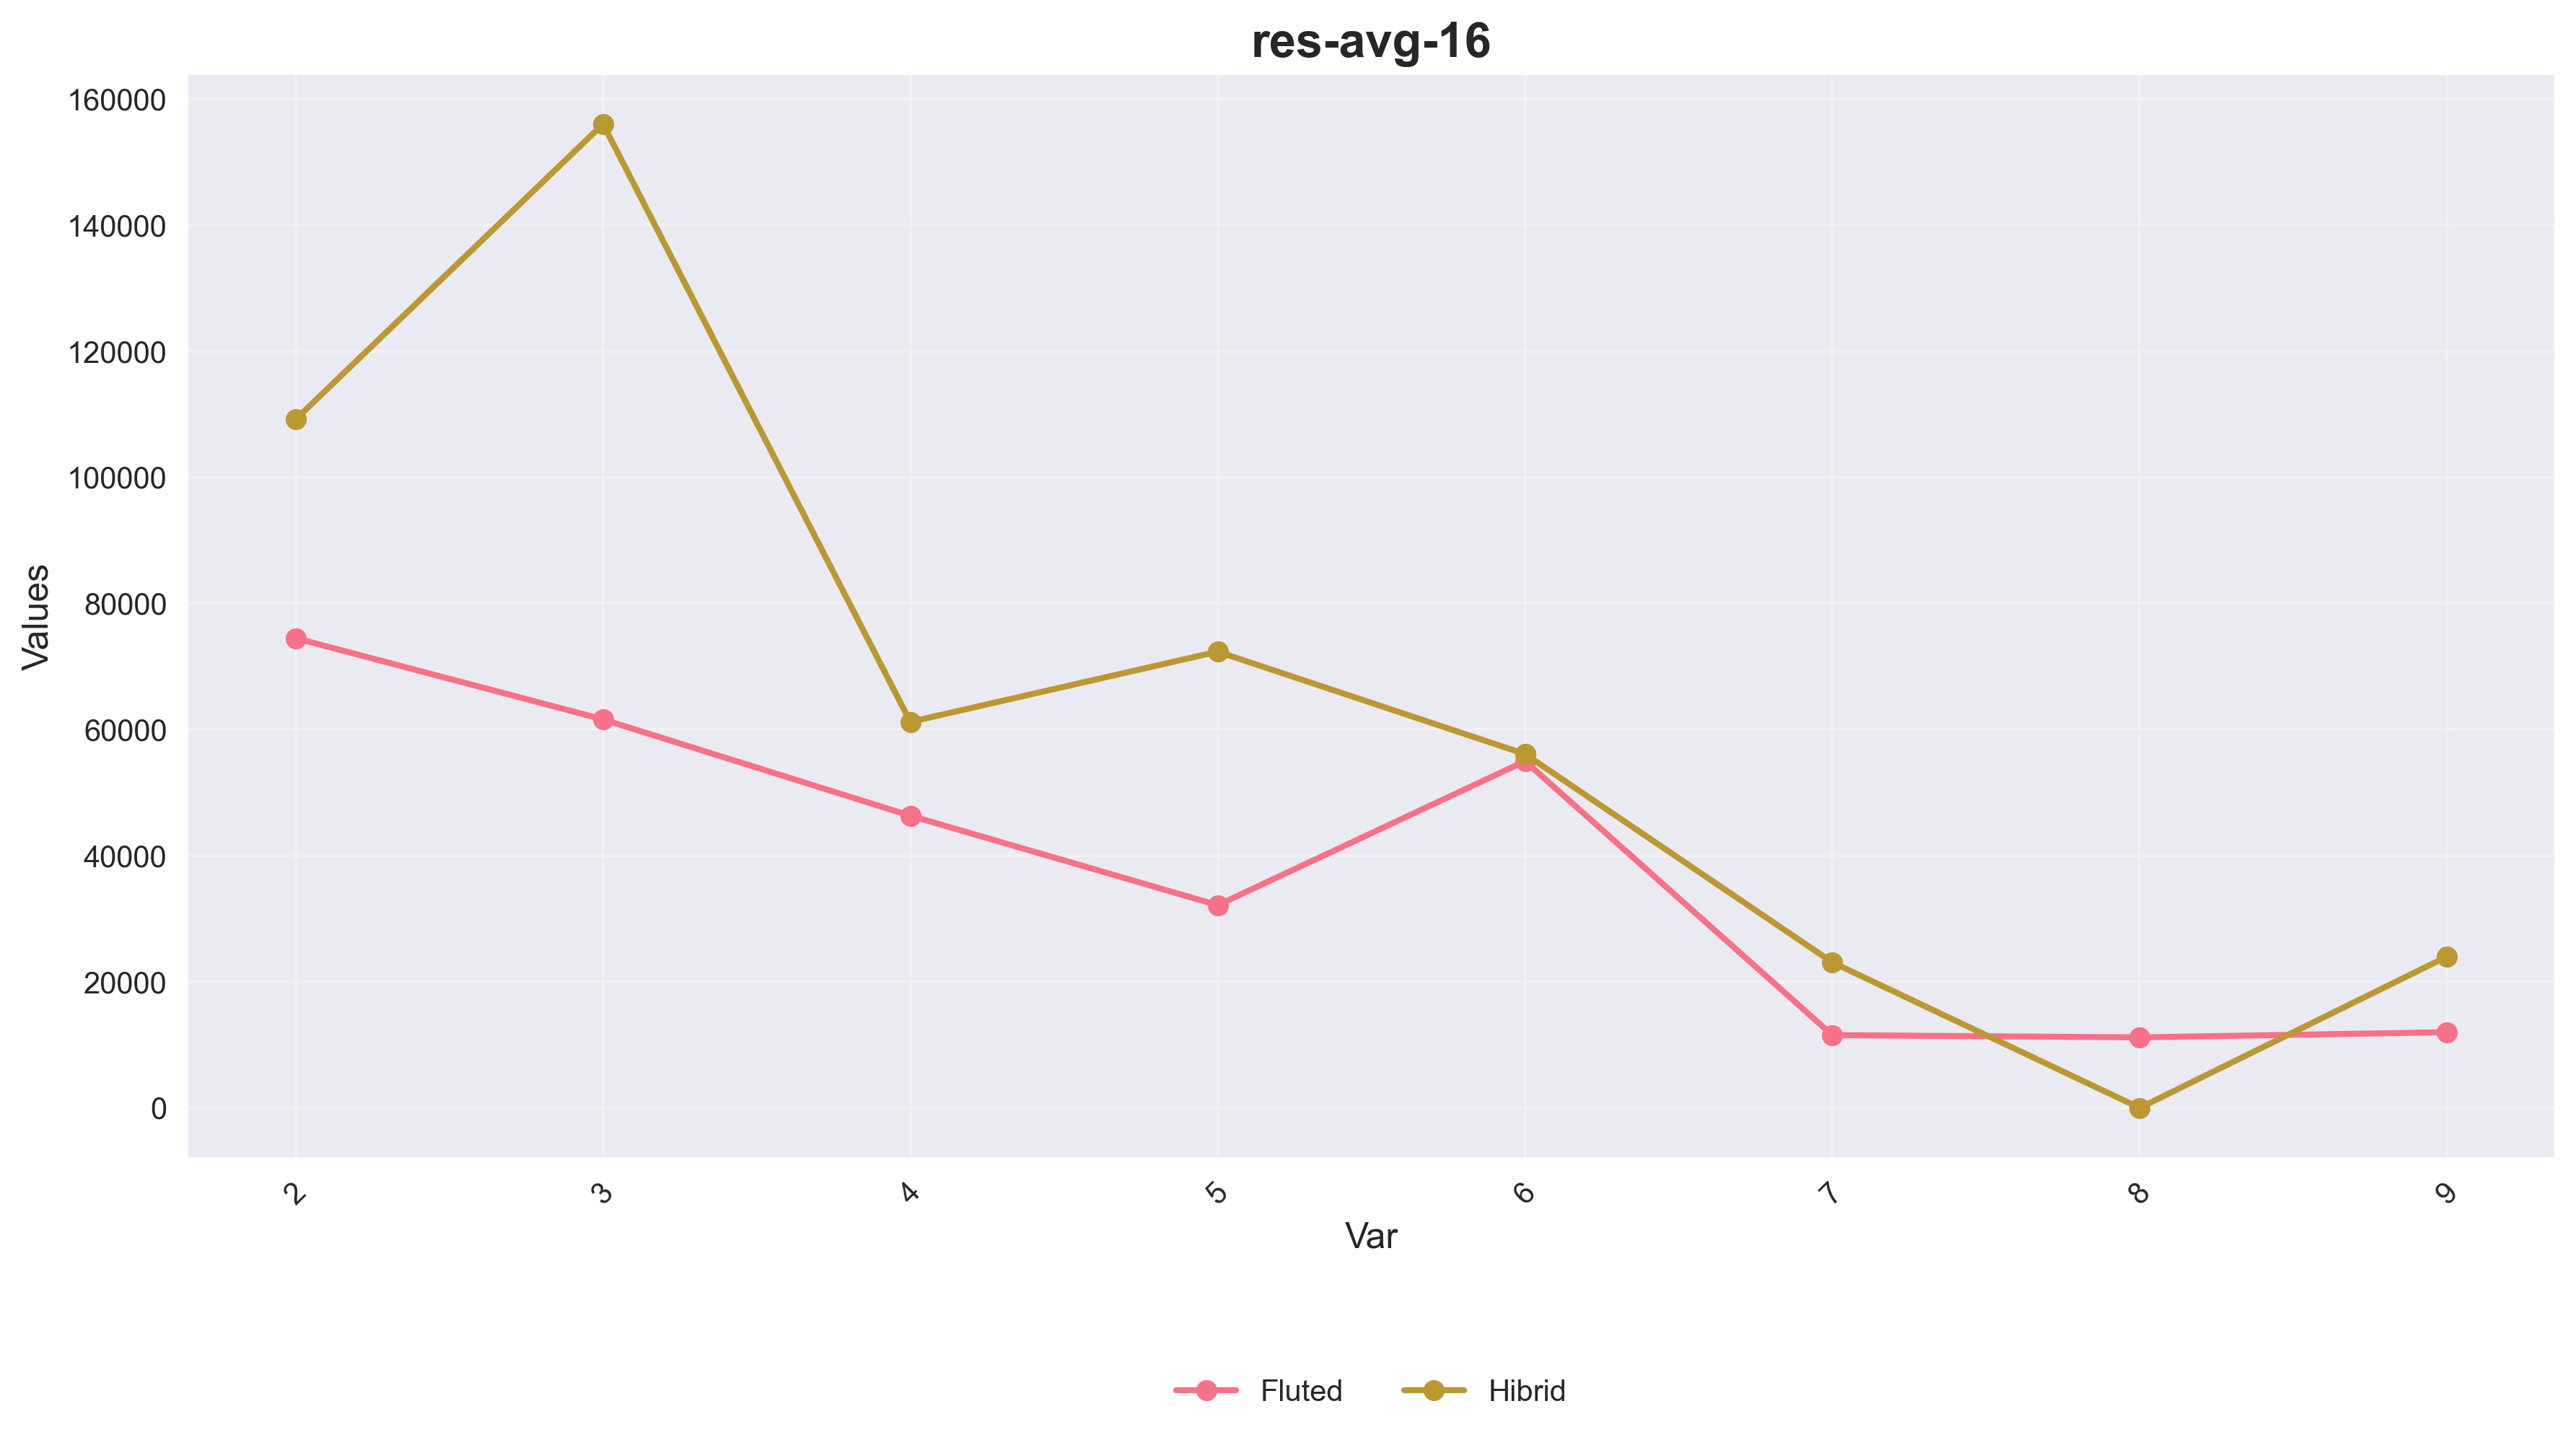
\includegraphics[width=\textwidth]{7-generated-benchmarking/aggregated/res-avg-16_linee_normal.png}
  \end{minipage}
  \caption{Aggregated results for generated problems with lexicographic encoding 16.}\label{fig:agg-le16}
\end{figure}

\begin{figure}[H]
  \centering
  \begin{minipage}{1\textwidth}
    \centering
    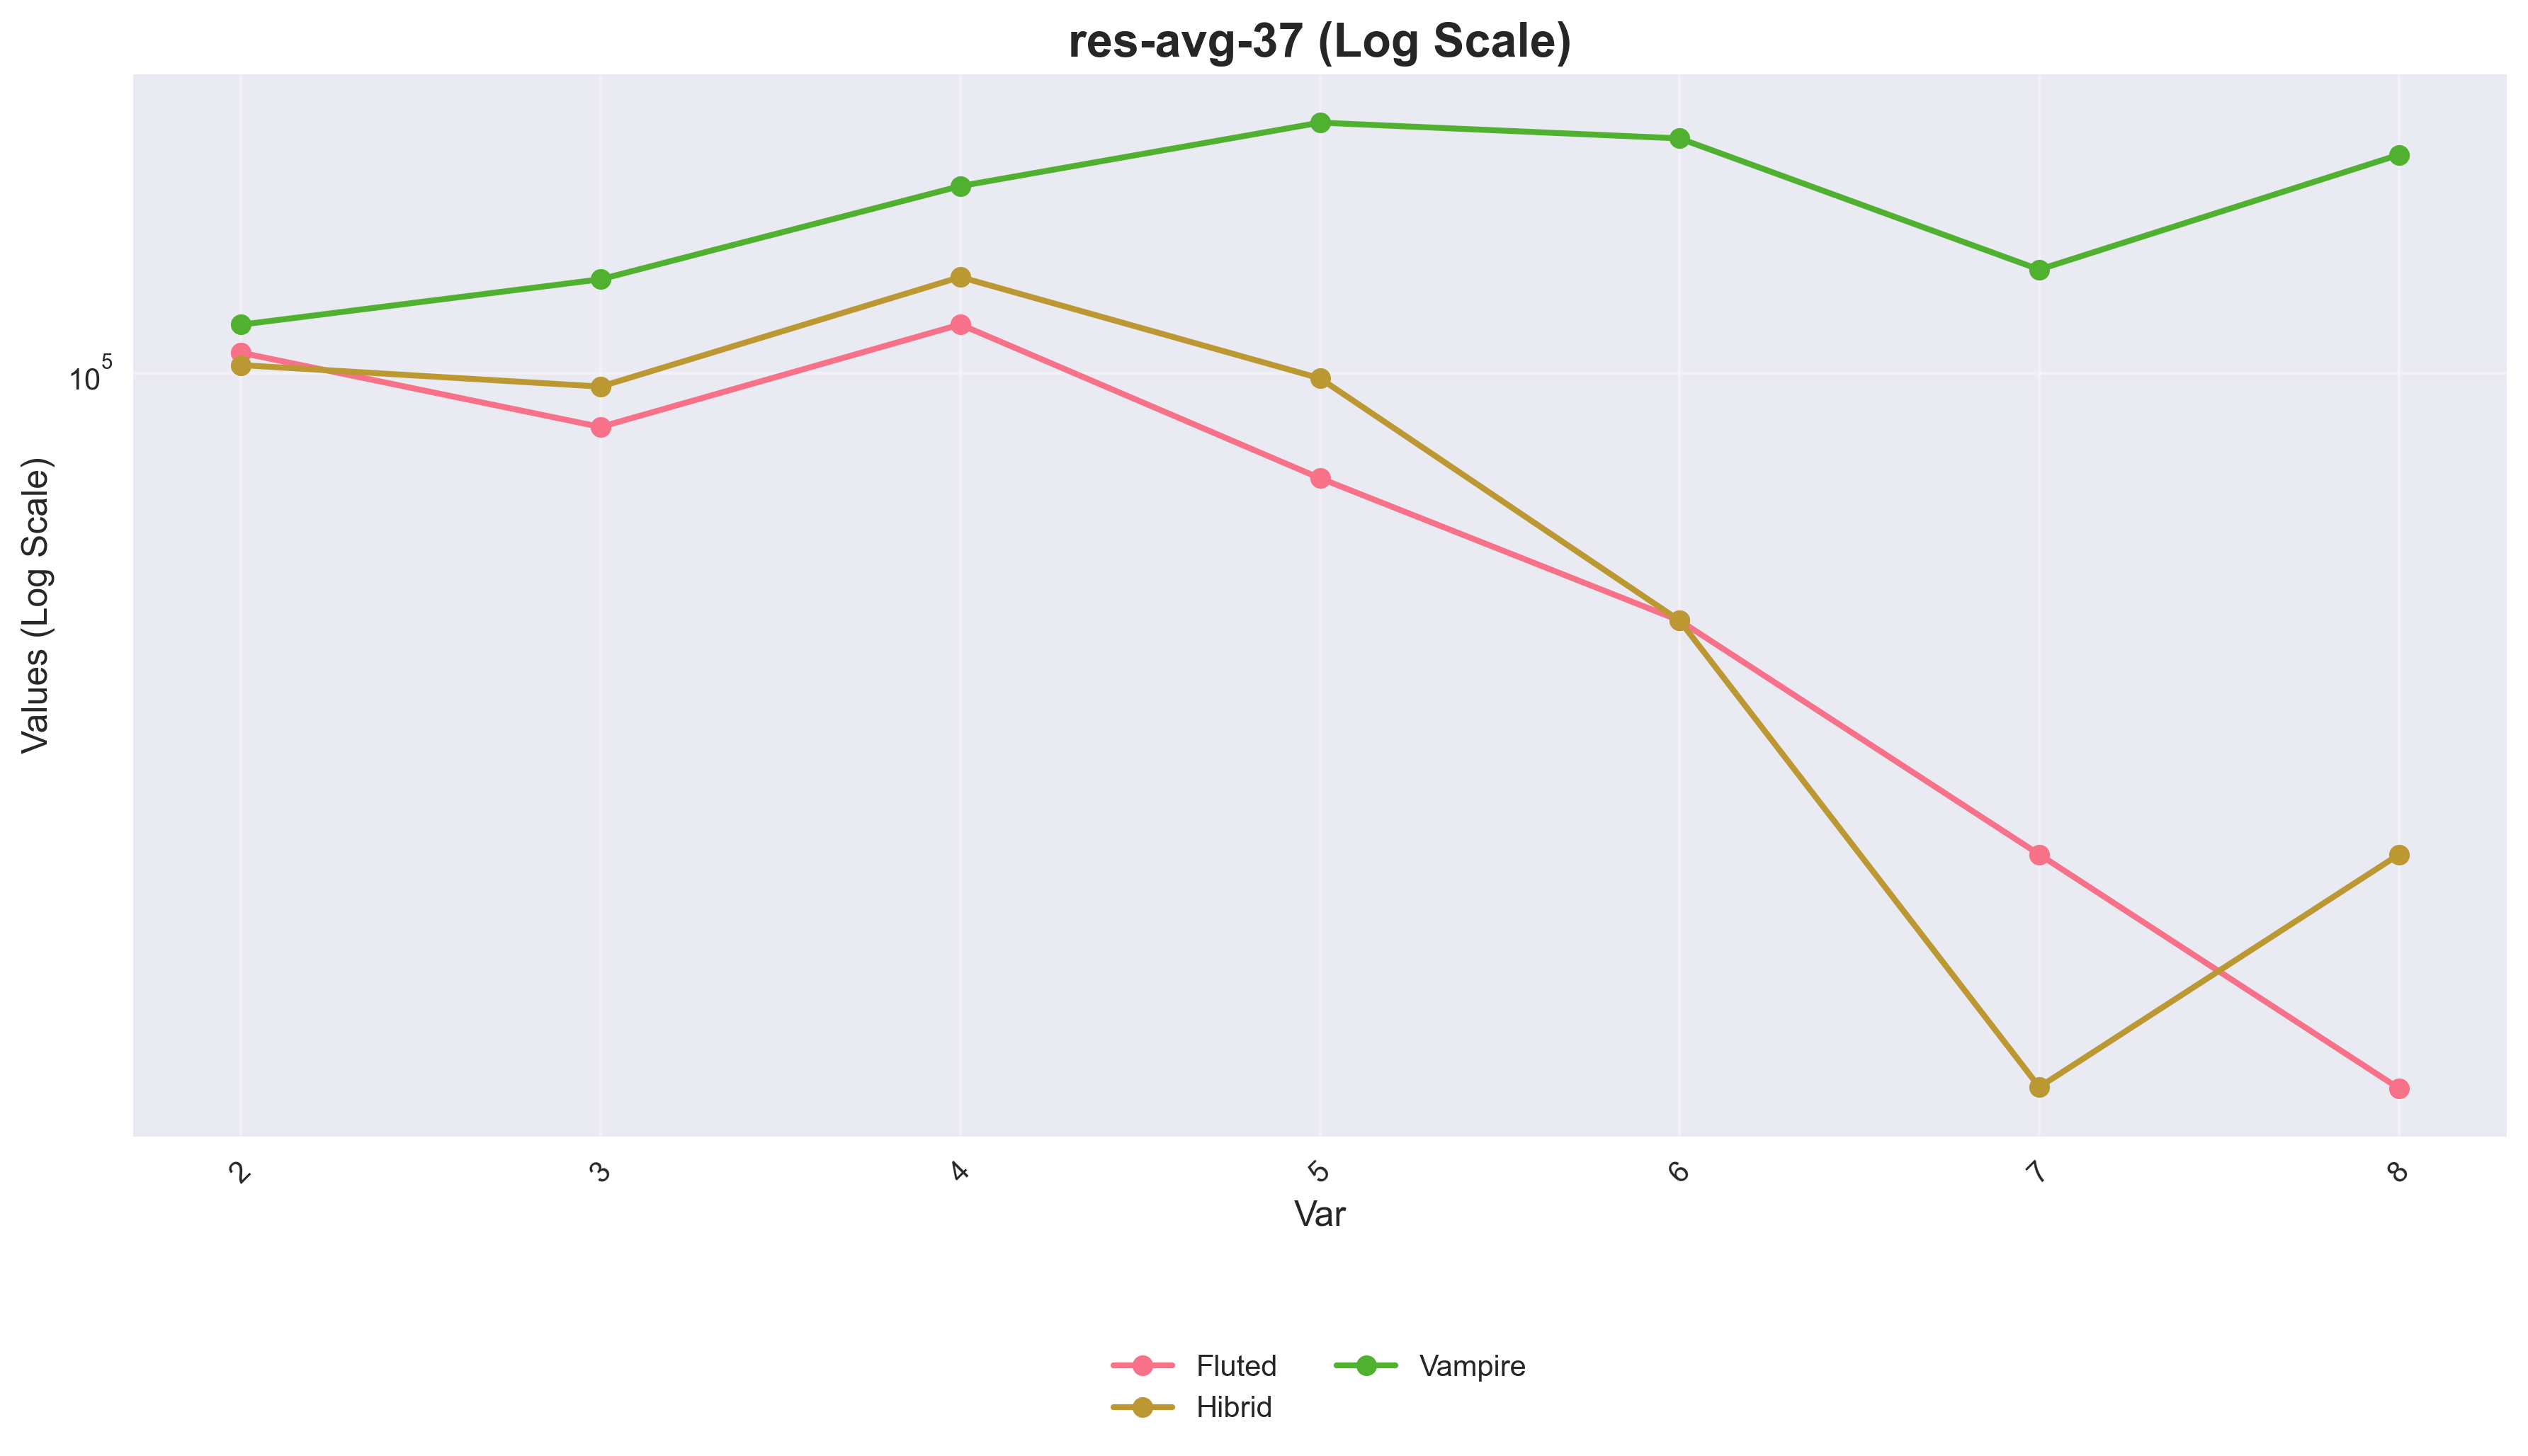
\includegraphics[width=\textwidth]{7-generated-benchmarking/aggregated/res-avg-37_linee_log.png}
  \end{minipage}
  \hfill
  \begin{minipage}{1\textwidth}
    \centering
    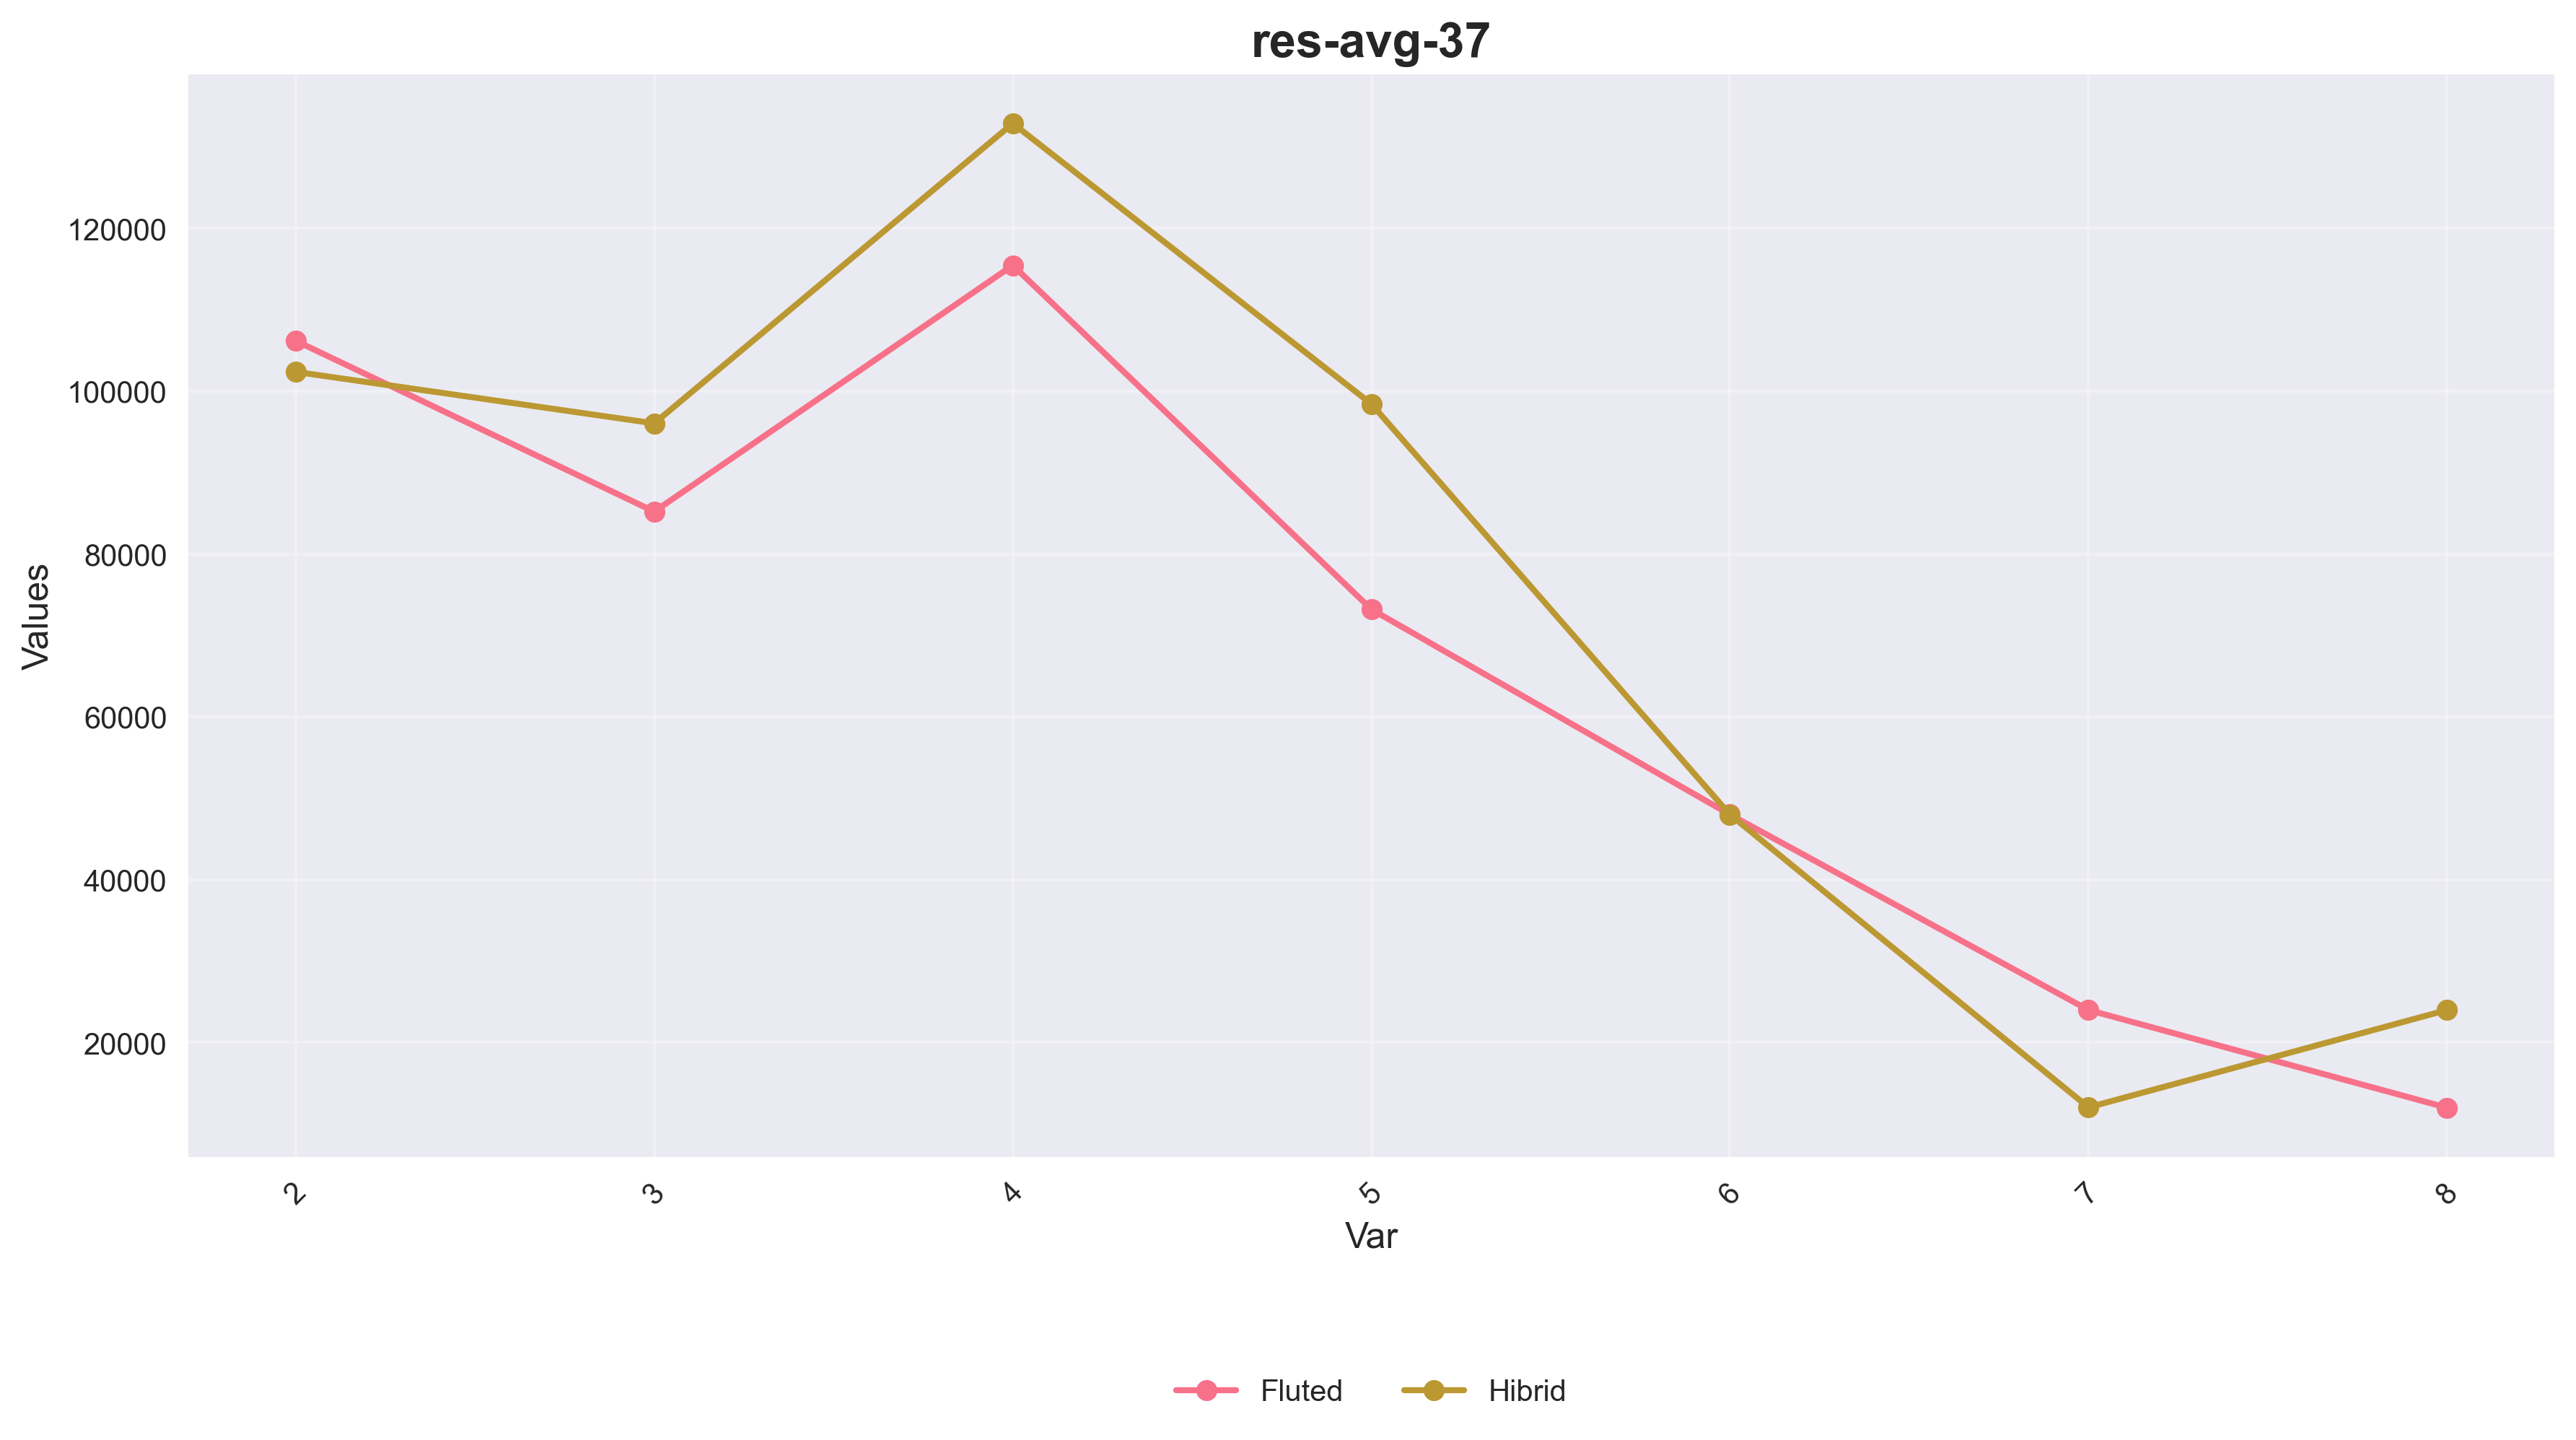
\includegraphics[width=\textwidth]{7-generated-benchmarking/aggregated/res-avg-37_linee_normal.png}
  \end{minipage}
  \caption{Aggregated results for generated problems with lexicographic encoding 37.}\label{fig:agg-le37}
\end{figure}

\begin{figure}[H]
  \centering
  \begin{minipage}{1\textwidth}
    \centering
    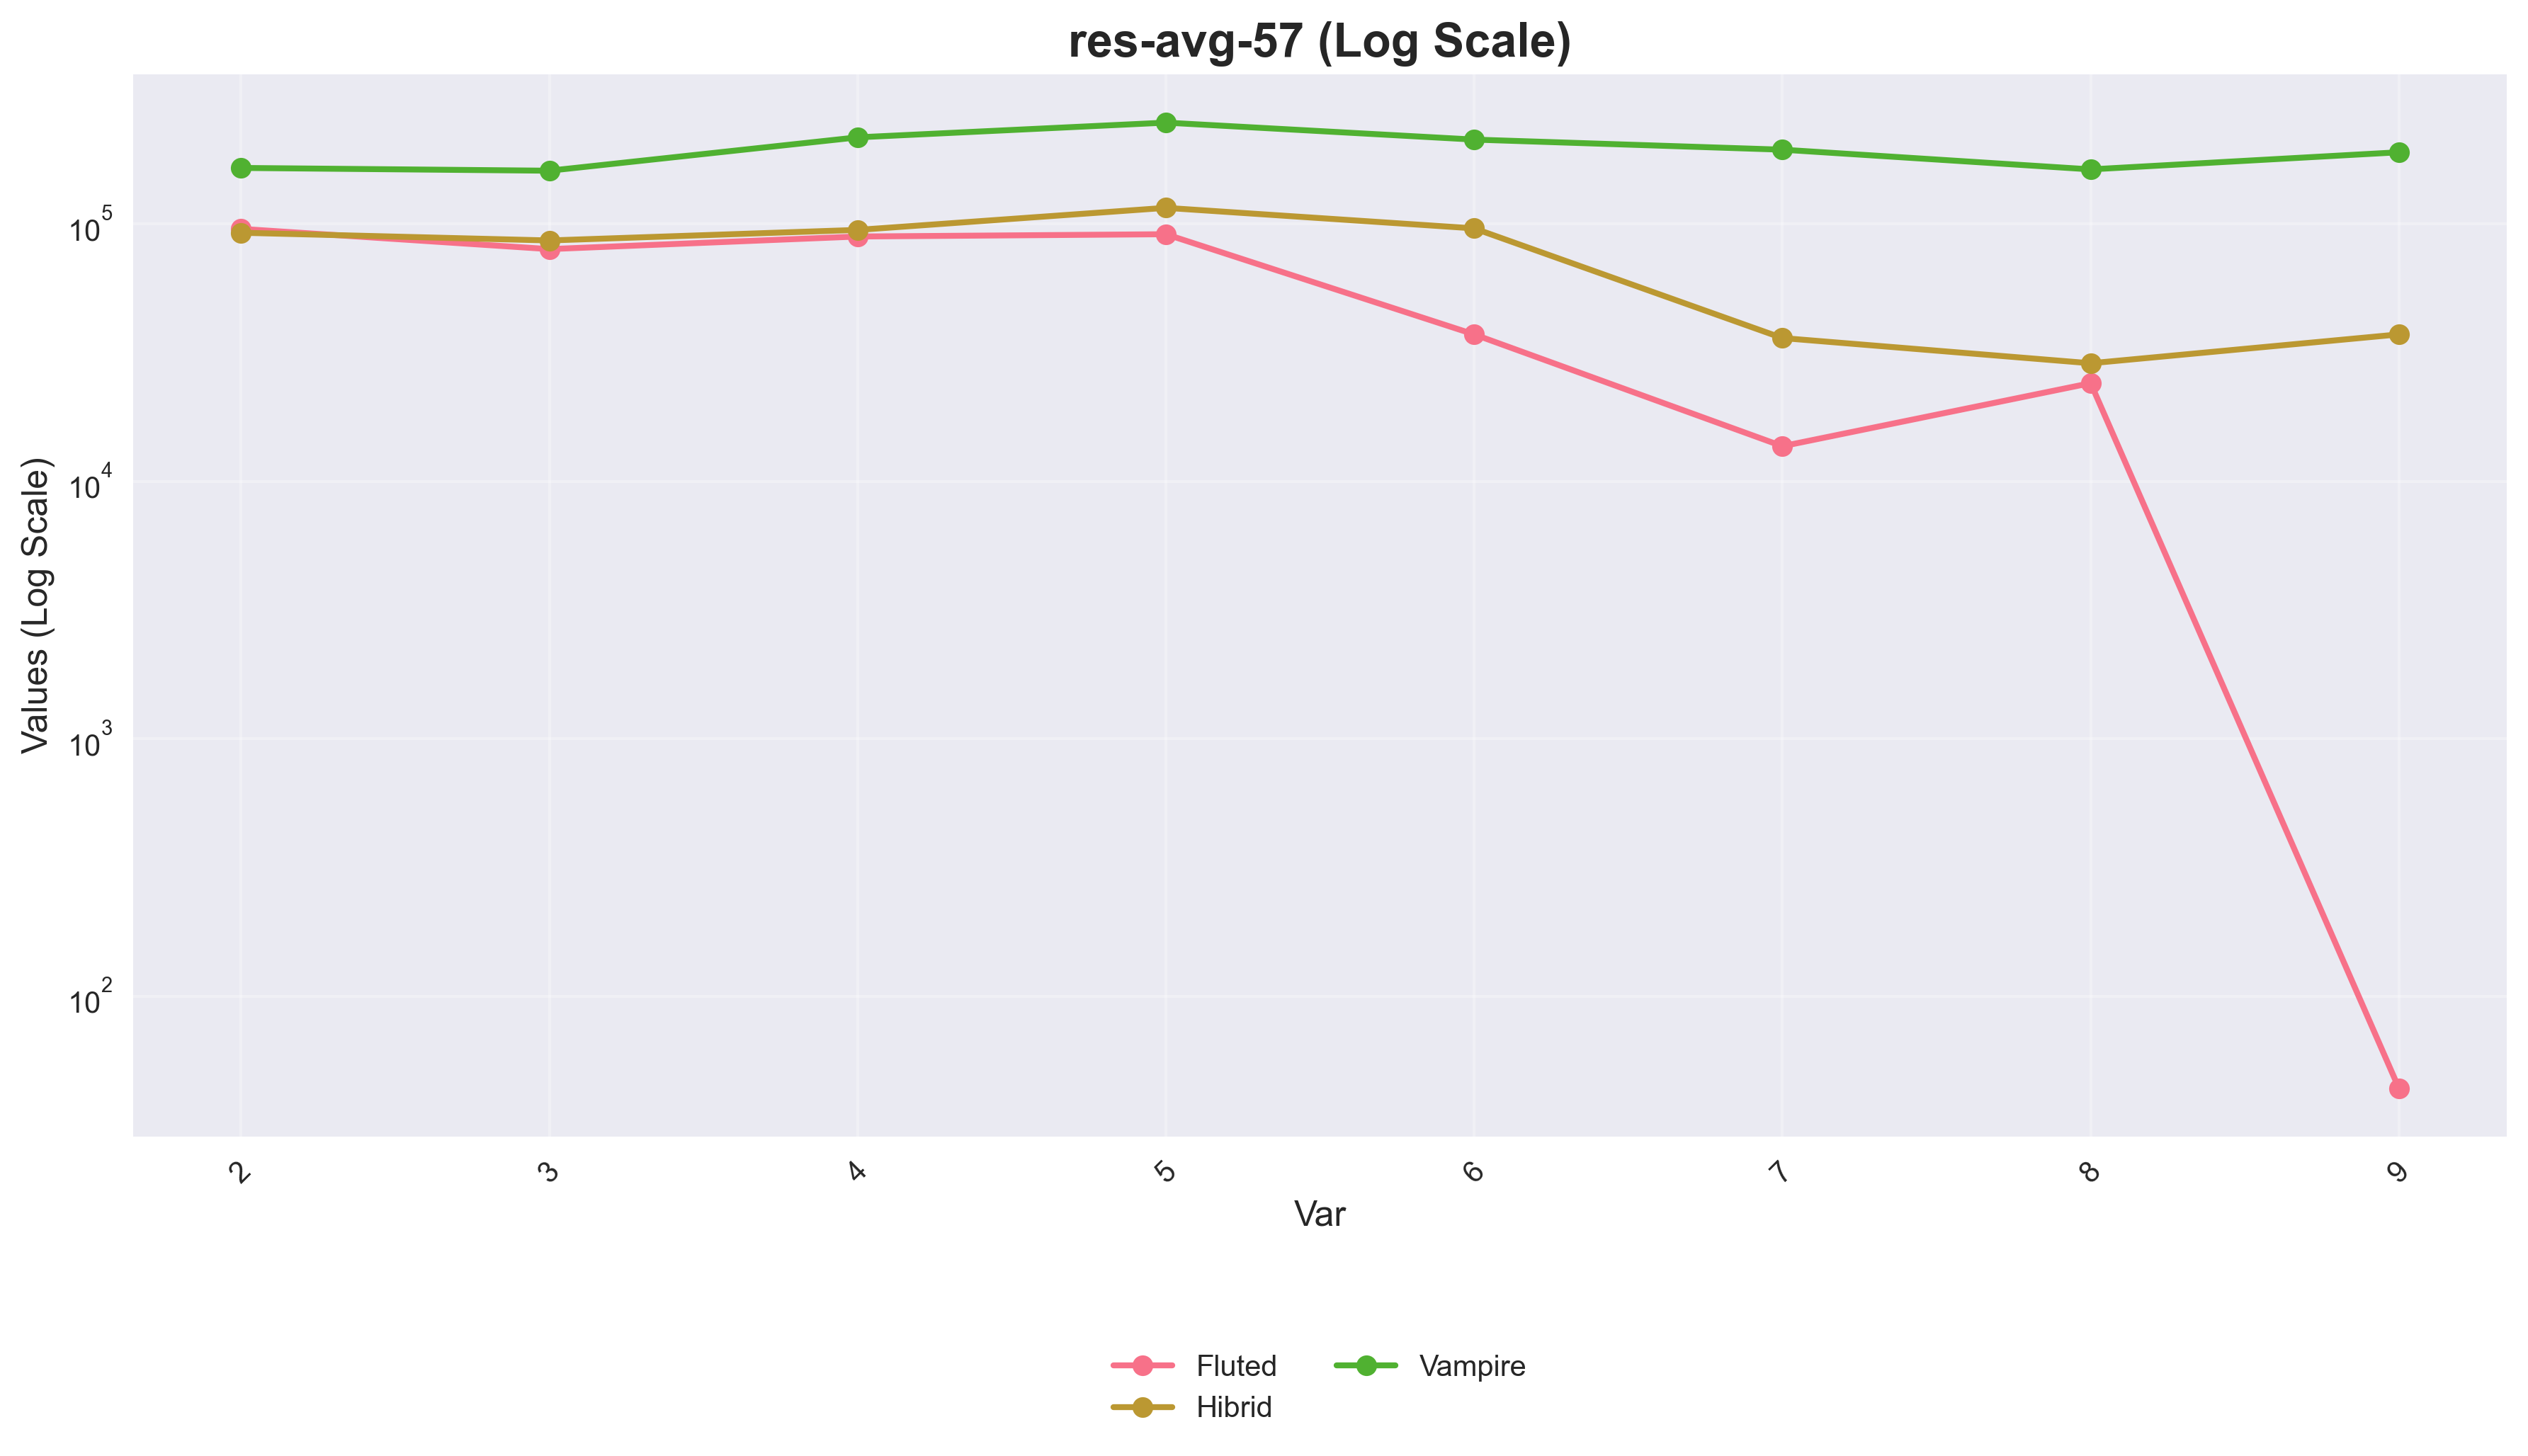
\includegraphics[width=\textwidth]{7-generated-benchmarking/aggregated/res-avg-57_linee_log.png}
  \end{minipage}
  \hfill
  \begin{minipage}{1\textwidth}
    \centering
    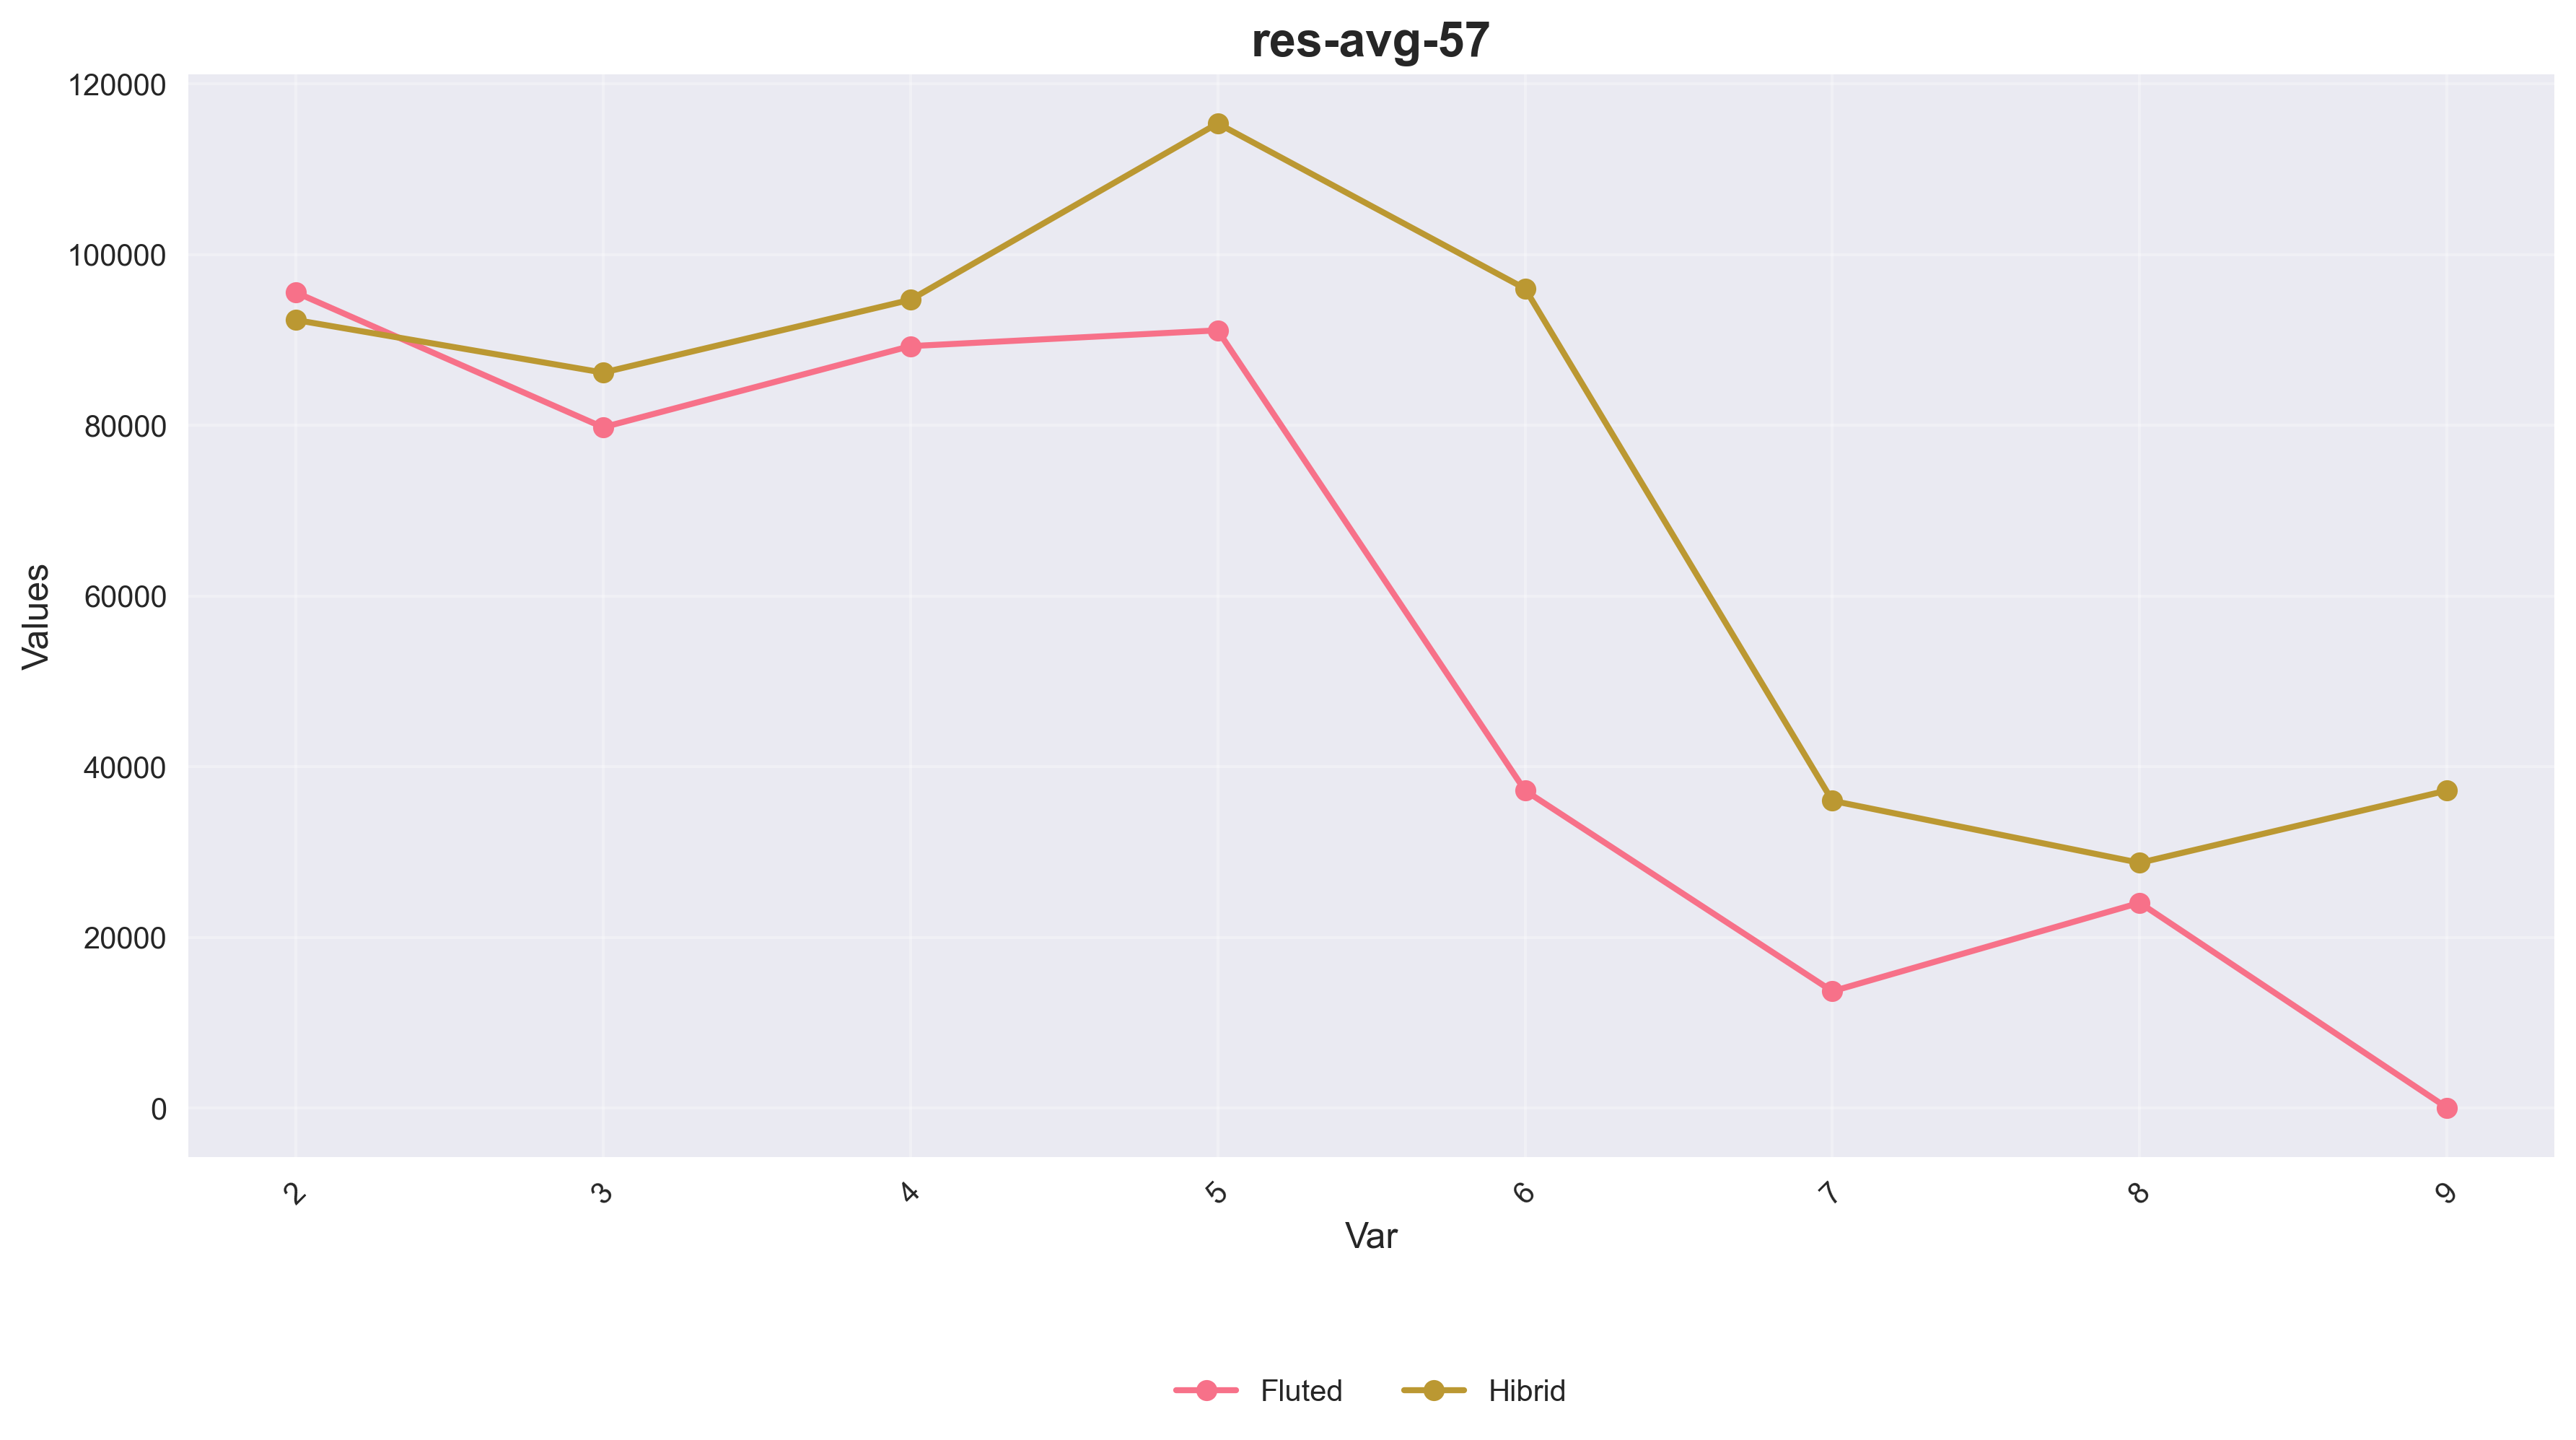
\includegraphics[width=\textwidth]{7-generated-benchmarking/aggregated/res-avg-57_linee_normal.png}
  \end{minipage}
  \caption{Aggregated results for generated problems with lexicographic encoding 57.}\label{fig:agg-le57}
\end{figure}

\begin{figure}[H]
  \centering
  \begin{minipage}{1\textwidth}
    \centering
    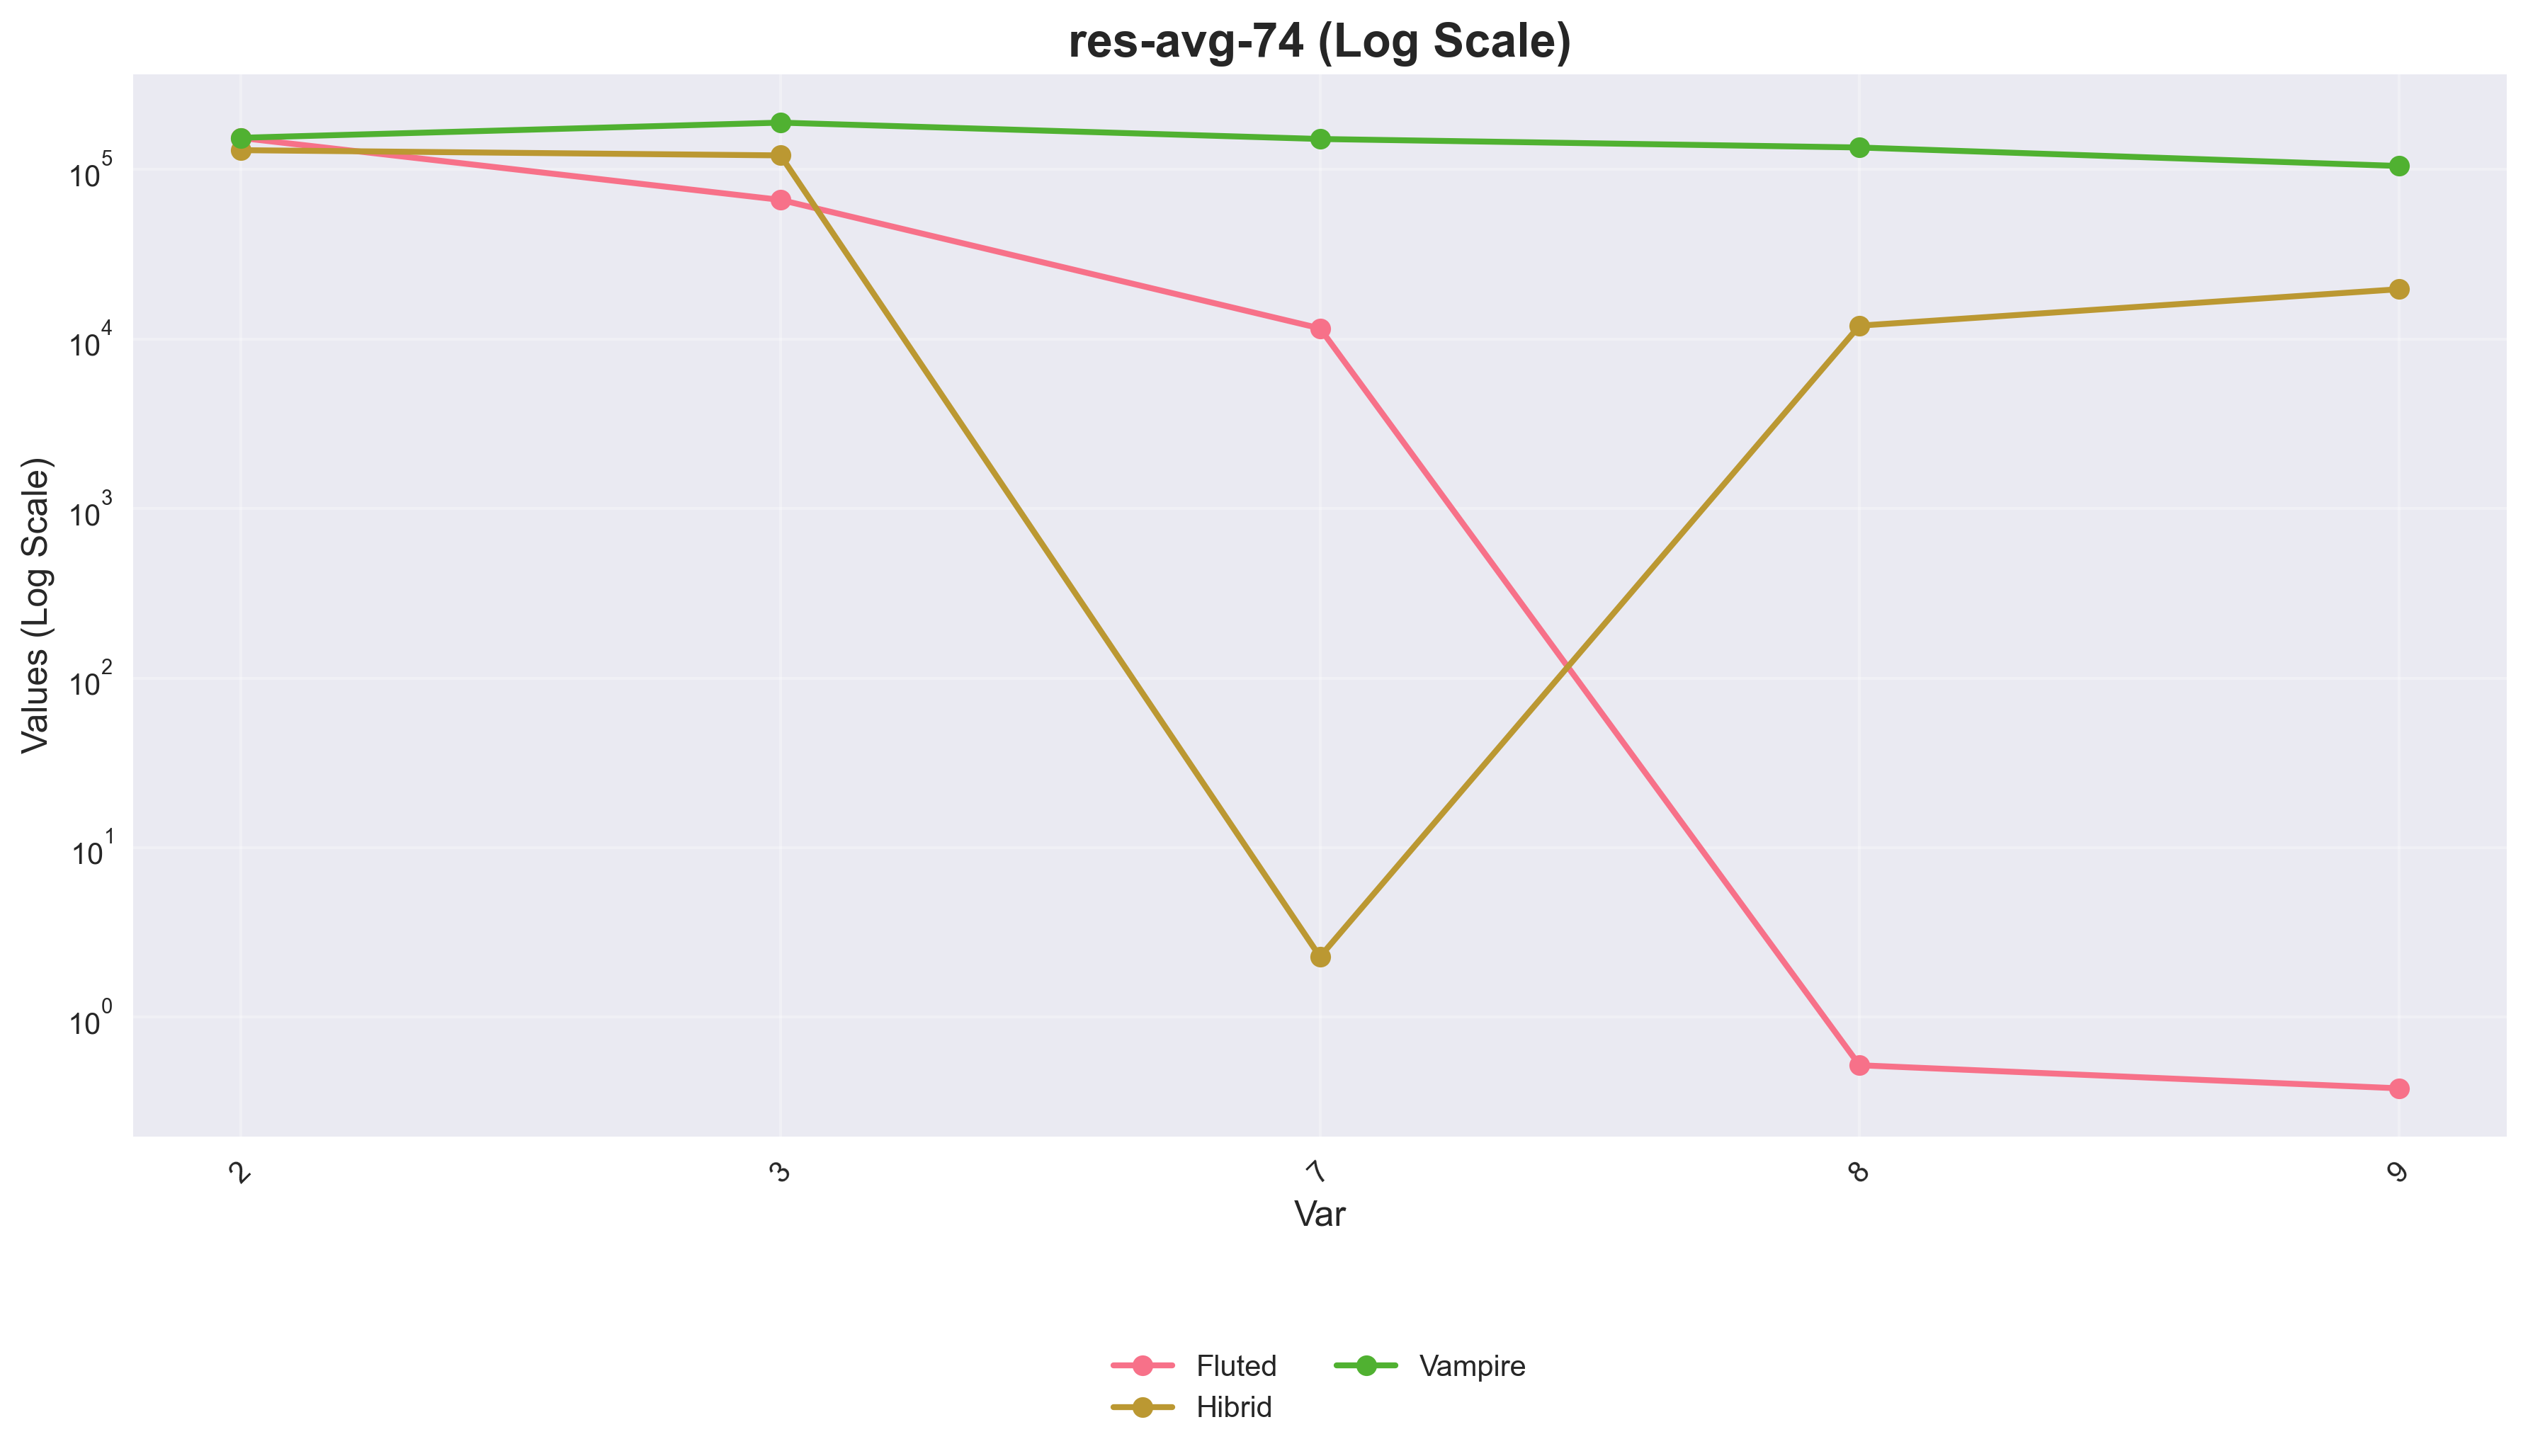
\includegraphics[width=\textwidth]{7-generated-benchmarking/aggregated/res-avg-74_linee_log.png}
  \end{minipage}
  \hfill
  \begin{minipage}{1\textwidth}
    \centering
    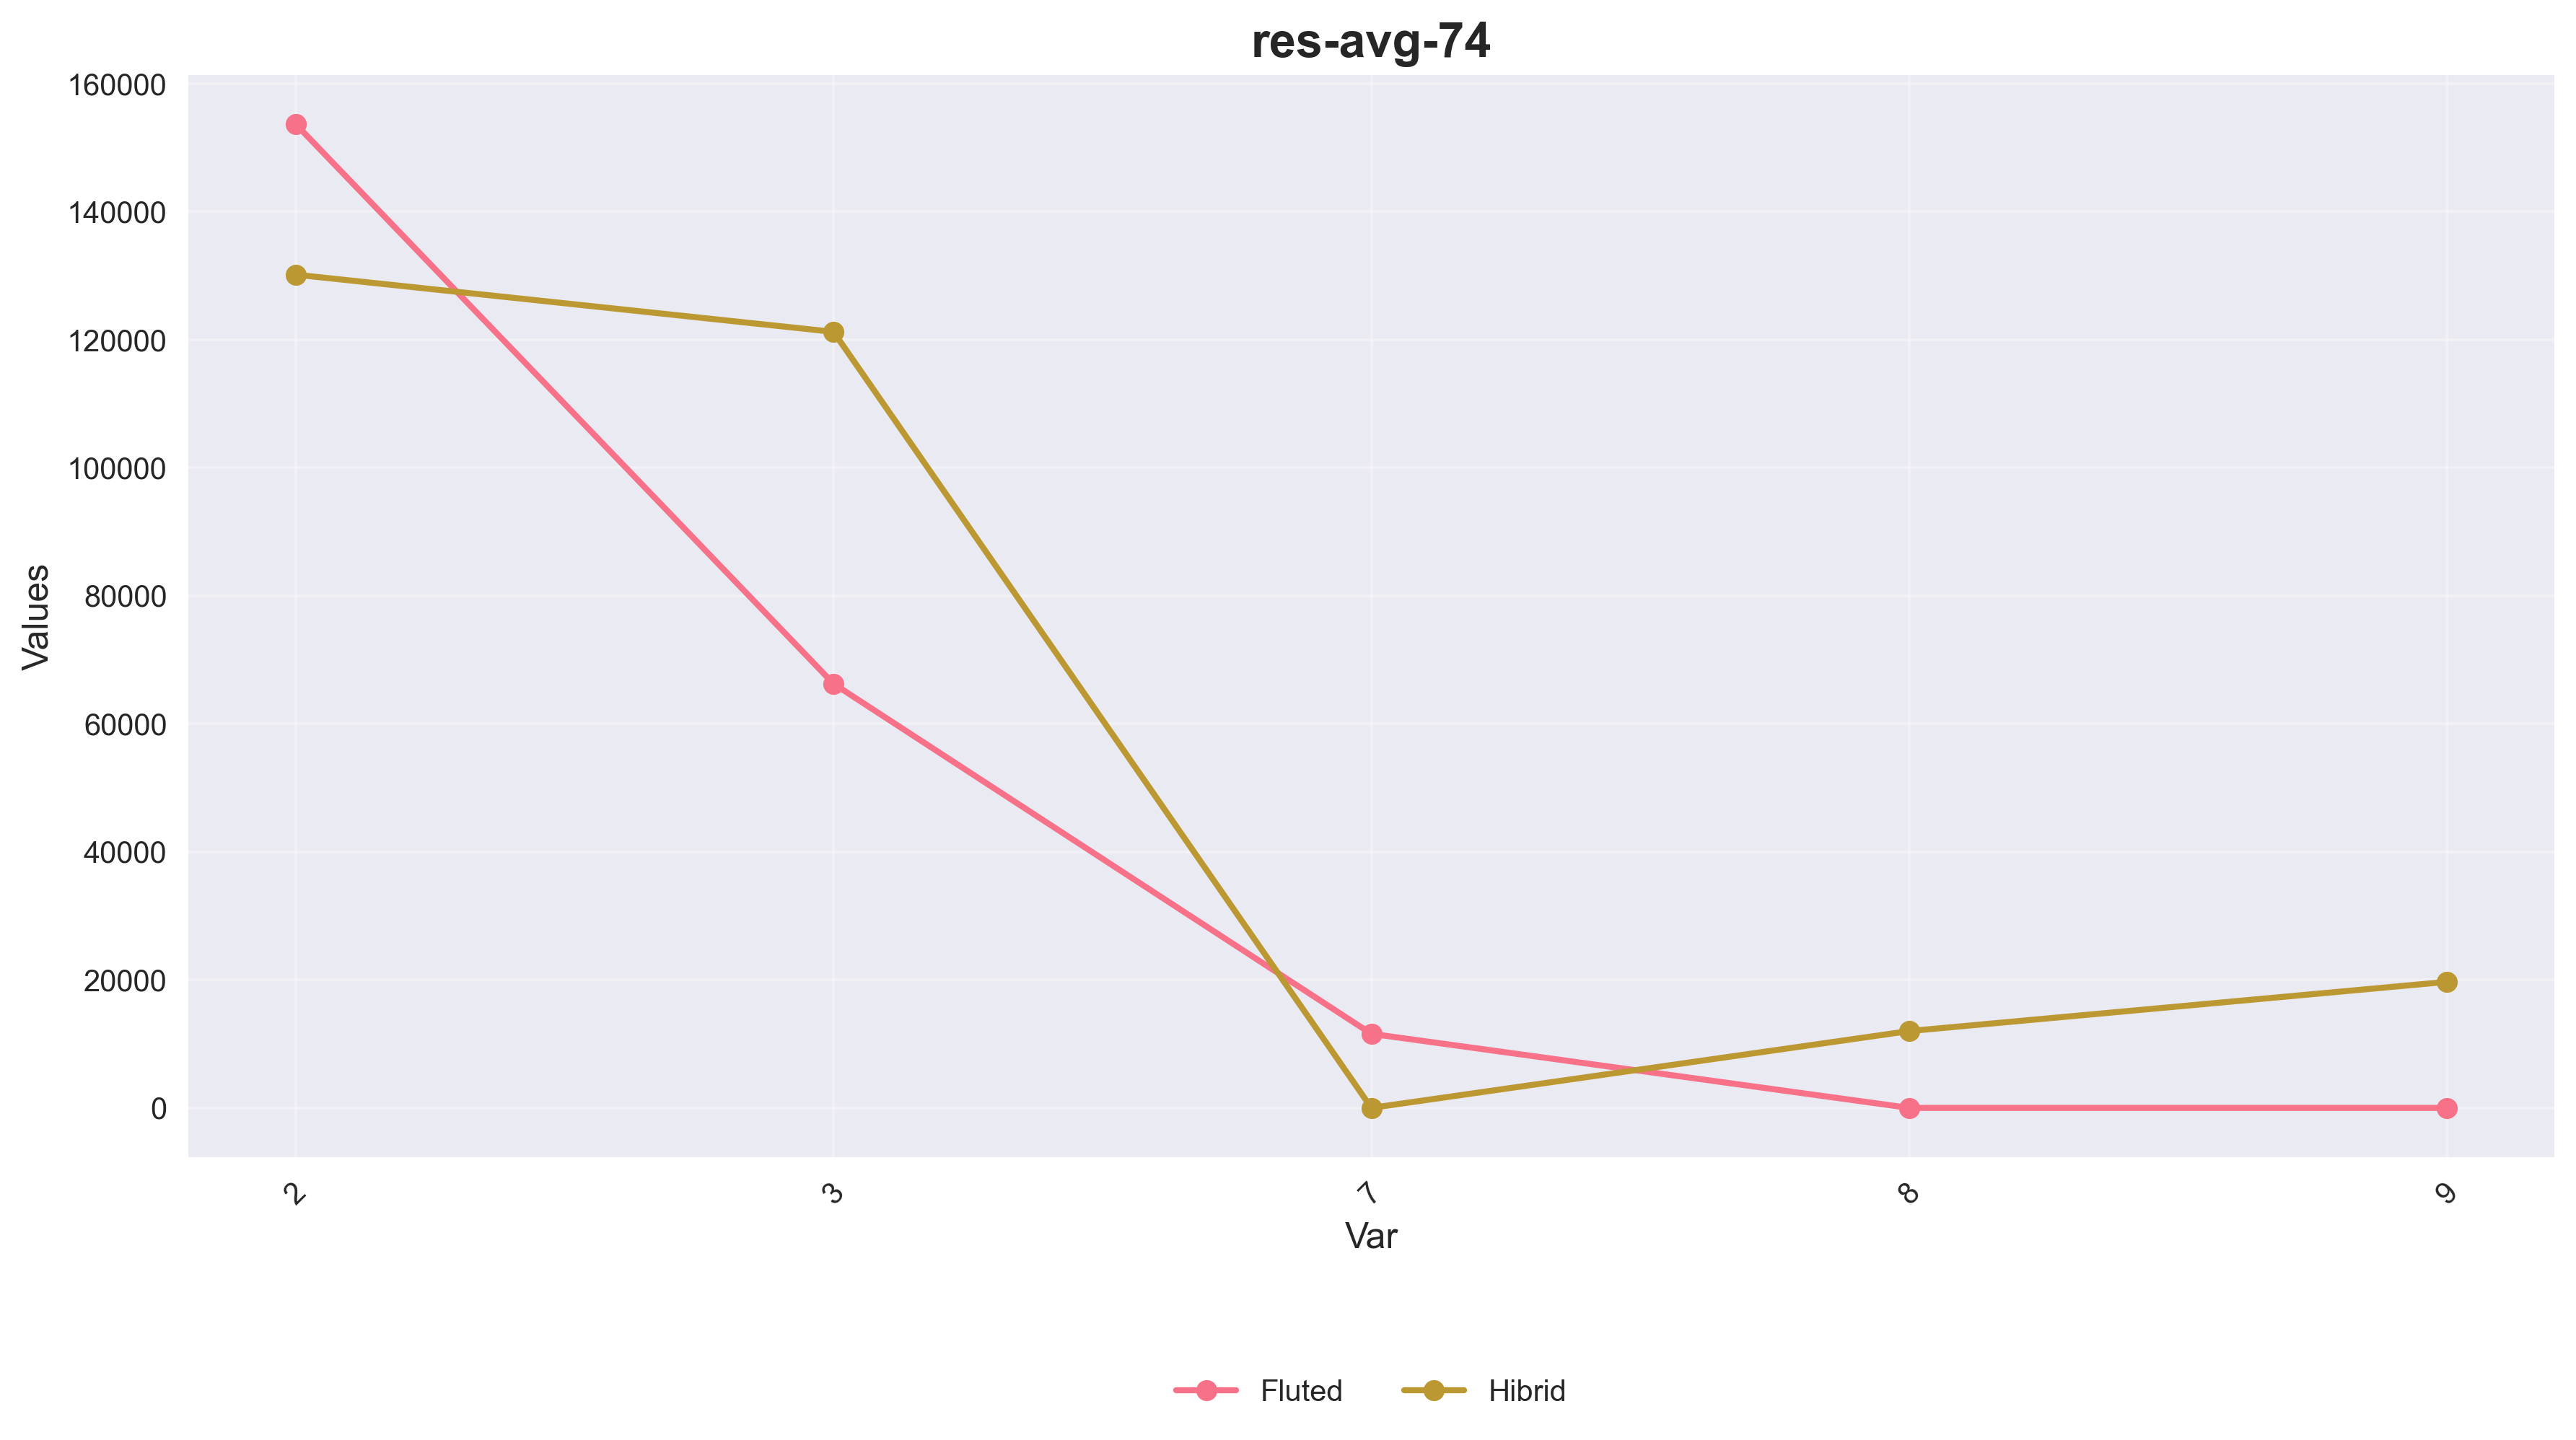
\includegraphics[width=\textwidth]{7-generated-benchmarking/aggregated/res-avg-74_linee_normal.png}
  \end{minipage}
  \caption{Aggregated results for generated problems with lexicographic encoding 74.}\label{fig:agg-le74}
\end{figure}

These charts already start to reveal some surprising trends. For confirmation, we averaged the results over all values of the other three parameters, leading to the final chart shown in Figure~\ref{fig:agg-all-vars}.
\begin{figure}[H]
  \centering
  \begin{minipage}{1\textwidth}
    \centering
    \includegraphics[width=\textwidth]{7-generated-benchmarking/aggregated/res-avg_linee_log.png}
  \end{minipage}
  \hfill
  \begin{minipage}{1\textwidth}
    \centering
    \includegraphics[width=\textwidth]{7-generated-benchmarking/aggregated/res-avg_linee_normal.png}
  \end{minipage}
  \caption{Aggregated results for generated problems over all values of \code{_predNum}, \code{_maxLen}, and \code{_unitsNum}.}\label{fig:agg-all-vars}
\end{figure}
From theoretical expectations, we would anticipate a significant increase in resolution time as the number of variables increases, given the non-elementary complexity associated with the fluted fragment.
However, the charts tell a different story. The performance seems to improve or remain relatively stable as the number of variables increases, which is counterintuitive.
This unexpected trend could be attributed to several factors, mainly related to some biases in the problem generation process.
Our hypothesis is that as the number of variables increases, less room is left for connectives and literals, leading to simpler formulae that are easier to resolve.
For example, with a maximum length of \(10\) and \(2\) variables, a formula have still \(8\) slots left, while with \(8\) variables, only \(2\) slots are left.
For solving this riddle, more in-depth analysis and testing would be required, possibly involving a more sophisticated problem generation process that can better control the complexity of the generated formulae independently of the number of variables.
An example of improvement could be to not count the quantifiers in the length of the formula (or at least the initial sequence of quantifiers), to avoid that increasing the number of variables directly decreases the number of other components in the formula.


